%!TEX spellcheck
%!TEX jobname = ti3allinone
%!TEX output_directory = out
%%%%%%%%%%%%%%%%%%%%%%%%%%%%%%%%%%%%%%%%%
%  My documentation report
%  Objetive: Explain what I did and how, so someone can continue with the investigation
%
% Important note:
% Chapter heading images should have a 2:1 width:height ratio,
% e.g. 920px width and 460px height.
%
%%%%%%%%%%%%%%%%%%%%%%%%%%%%%%%%%%%%%%%%%

%----------------------------------------------------------------------------------------
%	PACKAGES AND OTHER DOCUMENT CONFIGURATIONS
%----------------------------------------------------------------------------------------

\documentclass[11pt,fleqn]{book} % Default font size and left-justified equations

\usepackage[top=3cm,bottom=3cm,left=3.2cm,right=3.2cm,headsep=10pt,letterpaper]{geometry} % Page margins

\usepackage{xcolor} % Required for specifying colors by name
\definecolor{ocre}{RGB}{80,130,201} % Define the orange color used for highlighting throughout the book

% Font Settings
\usepackage{avant} % Use the Avantgarde font for headings
%\usepackage{times} % Use the Times font for headings
\usepackage{mathptmx} % Use the Adobe Times Roman as the default text font together with math symbols from the Sym­bol, Chancery and Com­puter Modern fonts

\usepackage{microtype} % Slightly tweak font spacing for aesthetics
\usepackage[utf8]{inputenc} % Required for including letters with accents
\usepackage[T1]{fontenc} % Use 8-bit encoding that has 256 glyphs

% Bibliography
% \usepackage[style=alphabetic,sorting=nyt,sortcites=true,autopunct=true,babel=hyphen,hyperref=true,abbreviate=false,backref=true,backend=biber]{biblatex}
% \addbibresource{bibliography.bib} % BibTeX bibliography file
% \defbibheading{bibempty}{}

%----------------------------------------------------------------------------------------
%	VARIOUS REQUIRED PACKAGES
%----------------------------------------------------------------------------------------

\usepackage{titlesec} % Allows customization of titles

\usepackage{graphicx} % Required for including pictures
\graphicspath{{Pictures/}} % Specifies the directory where pictures are stored

\usepackage{lipsum} % Inserts dummy text

\usepackage{tikz} % Required for drawing custom shapes

\usepackage[english]{babel} % English language/hyphenation

\usepackage{enumitem} % Customize lists
\setlist{nolistsep} % Reduce spacing between bullet points and numbered lists

\usepackage{booktabs} % Required for nicer horizontal rules in tables

\usepackage{eso-pic} % Required for specifying an image background in the title page

\usepackage{float}

%----------------------------------------------------------------------------------------
%	MAIN TABLE OF CONTENTS
%----------------------------------------------------------------------------------------

\usepackage{titletoc} % Required for manipulating the table of contents

\contentsmargin{0cm} % Removes the default margin
% Chapter text styling
\titlecontents{chapter}[1.25cm] % Indentation
{\addvspace{15pt}\large\sffamily\bfseries} % Spacing and font options for chapters
{\color{ocre!60}\contentslabel[\Large\thecontentslabel]{1.25cm}\color{ocre}} % Chapter number
{}  
{\color{ocre!60}\normalsize\sffamily\bfseries\;\titlerule*[.5pc]{.}\;\thecontentspage} % Page number
% Section text styling
\titlecontents{section}[1.25cm] % Indentation
{\addvspace{5pt}\sffamily\bfseries} % Spacing and font options for sections
{\contentslabel[\thecontentslabel]{1.25cm}} % Section number
{}
{\sffamily\hfill\color{black}\thecontentspage} % Page number
[]
% Subsection text styling
\titlecontents{subsection}[1.25cm] % Indentation
{\addvspace{1pt}\sffamily\small} % Spacing and font options for subsections
{\contentslabel[\thecontentslabel]{1.25cm}} % Subsection number
{}
{\sffamily\;\titlerule*[.5pc]{.}\;\thecontentspage} % Page number
[] 

%----------------------------------------------------------------------------------------
%	MINI TABLE OF CONTENTS IN CHAPTER HEADS
%----------------------------------------------------------------------------------------

% Section text styling
\titlecontents{lsection}[0em] % Indendating
{\footnotesize\sffamily} % Font settings
{}
{}
{}

% Subsection text styling
\titlecontents{lsubsection}[.5em] % Indentation
{\normalfont\footnotesize\sffamily} % Font settings
{}
{}
{}
 
%----------------------------------------------------------------------------------------
%	PAGE HEADERS
%----------------------------------------------------------------------------------------

\usepackage{fancyhdr} % Required for header and footer configuration

\pagestyle{fancy}
\renewcommand{\chaptermark}[1]{\markboth{\sffamily\normalsize\bfseries\chaptername\ \thechapter.\ #1}{}} % Chapter text font settings
\renewcommand{\sectionmark}[1]{\markright{\sffamily\normalsize\thesection\hspace{5pt}#1}{}} % Section text font settings
\fancyhf{} \fancyhead[LE,RO]{\sffamily\normalsize\thepage} % Font setting for the page number in the header
\fancyhead[LO]{\rightmark} % Print the nearest section name on the left side of odd pages
\fancyhead[RE]{\leftmark} % Print the current chapter name on the right side of even pages
\renewcommand{\headrulewidth}{0.5pt} % Width of the rule under the header
\addtolength{\headheight}{2.5pt} % Increase the spacing around the header slightly
\renewcommand{\footrulewidth}{0pt} % Removes the rule in the footer
\fancypagestyle{plain}{\fancyhead{}\renewcommand{\headrulewidth}{0pt}} % Style for when a plain pagestyle is specified

% Removes the header from odd empty pages at the end of chapters
\makeatletter
\renewcommand{\cleardoublepage}{
\clearpage\ifodd\c@page\else
\hbox{}
\vspace*{\fill}
\thispagestyle{empty}
\newpage
\fi}

%----------------------------------------------------------------------------------------
%	THEOREM STYLES
%----------------------------------------------------------------------------------------

\usepackage{amsmath,amsfonts,amssymb,amsthm} % For math equations, theorems, symbols, etc

\newcommand{\intoo}[2]{\mathopen{]}#1\,;#2\mathclose{[}}
\newcommand{\ud}{\mathop{\mathrm{{}d}}\mathopen{}}
\newcommand{\intff}[2]{\mathopen{[}#1\,;#2\mathclose{]}}
\newtheorem{notation}{Notation}[chapter]

%%%%%%%%%%%%%%%%%%%%%%%%%%%%%%%%%%%%%%%%%%%%%%%%%%%%%%%%%%%%%%%%%%%%%%%%%%%
%%%%%%%%%%%%%%%%%%%% dedicated to boxed/framed environements %%%%%%%%%%%%%%
%%%%%%%%%%%%%%%%%%%%%%%%%%%%%%%%%%%%%%%%%%%%%%%%%%%%%%%%%%%%%%%%%%%%%%%%%%%
\newtheoremstyle{ocrenumbox}% % Theorem style name
{0pt}% Space above
{0pt}% Space below
{\normalfont}% % Body font
{}% Indent amount
{\small\bf\sffamily\color{ocre}}% % Theorem head font
{\;}% Punctuation after theorem head
{0.25em}% Space after theorem head
{\small\sffamily\color{ocre}\thmname{#1}\nobreakspace\thmnumber{\@ifnotempty{#1}{}\@upn{#2}}% Theorem text (e.g. Theorem 2.1)
\thmnote{\nobreakspace\the\thm@notefont\sffamily\bfseries\color{black}---\nobreakspace#3.}} % Optional theorem note
\renewcommand{\qedsymbol}{$\blacksquare$}% Optional qed square

\newtheoremstyle{blacknumex}% Theorem style name
{5pt}% Space above
{5pt}% Space below
{\normalfont}% Body font
{} % Indent amount
{\small\bf\sffamily}% Theorem head font
{\;}% Punctuation after theorem head
{0.25em}% Space after theorem head
{\small\sffamily{\tiny\ensuremath{\blacksquare}}\nobreakspace\thmname{#1}\nobreakspace\thmnumber{\@ifnotempty{#1}{}\@upn{#2}}% Theorem text (e.g. Theorem 2.1)
\thmnote{\nobreakspace\the\thm@notefont\sffamily\bfseries---\nobreakspace#3.}}% Optional theorem note

\newtheoremstyle{blacknumbox} % Theorem style name
{0pt}% Space above
{0pt}% Space below
{\normalfont}% Body font
{}% Indent amount
{\small\bf\sffamily}% Theorem head font
{\;}% Punctuation after theorem head
{0.25em}% Space after theorem head
{\small\sffamily\thmname{#1}\nobreakspace\thmnumber{\@ifnotempty{#1}{}\@upn{#2}}% Theorem text (e.g. Theorem 2.1)
\thmnote{\nobreakspace\the\thm@notefont\sffamily\bfseries---\nobreakspace#3.}}% Optional theorem note

%%%%%%%%%%%%%%%%%%%%%%%%%%%%%%%%%%%%%%%%%%%%%%%%%%%%%%%%%%%%%%%%%%%%%%%%%%%
%%%%%%%%%%%%% dedicated to non-boxed/non-framed environements %%%%%%%%%%%%%
%%%%%%%%%%%%%%%%%%%%%%%%%%%%%%%%%%%%%%%%%%%%%%%%%%%%%%%%%%%%%%%%%%%%%%%%%%%
\newtheoremstyle{ocrenum}% % Theorem style name
{5pt}% Space above
{5pt}% Space below
{\normalfont}% % Body font
{}% Indent amount
{\small\bf\sffamily\color{ocre}}% % Theorem head font
{\;}% Punctuation after theorem head
{0.25em}% Space after theorem head
{\small\sffamily\color{ocre}\thmname{#1}\nobreakspace\thmnumber{\@ifnotempty{#1}{}\@upn{#2}}% Theorem text (e.g. Theorem 2.1)
\thmnote{\nobreakspace\the\thm@notefont\sffamily\bfseries\color{black}---\nobreakspace#3.}} % Optional theorem note
\renewcommand{\qedsymbol}{$\blacksquare$}% Optional qed square
\makeatother

% Defines the theorem text style for each type of theorem to one of the three styles above
\newcounter{dummy} 
\numberwithin{dummy}{section}
\theoremstyle{ocrenumbox}
\newtheorem{theoremeT}[dummy]{Theorem}
\newtheorem{problem}{Problem}[chapter]
\newtheorem{exerciseT}{Exercise}[chapter]
\theoremstyle{blacknumex}
\newtheorem{exampleT}{Example}[chapter]
\theoremstyle{blacknumbox}
\newtheorem{vocabulary}{Vocabulary}[chapter]
\newtheorem{definitionT}{Definition}[section]
\newtheorem{corollaryT}[dummy]{Corollary}
\theoremstyle{ocrenum}
\newtheorem{proposition}[dummy]{Proposition}

%----------------------------------------------------------------------------------------
%	
%----------------------------------------------------------------------------------------

\RequirePackage[framemethod=default]{mdframed} % Required for creating the theorem, definition, exercise and corollary boxes

\newmdenv[skipabove=7pt,
skipbelow=7pt,
rightline=false,
leftline=true,
topline=false,
bottomline=false,
backgroundcolor=blue!8,
linecolor=blue!80,
innerleftmargin=5pt,
innerrightmargin=5pt,
innertopmargin=5pt,
innerbottommargin=5pt,
leftmargin=0cm,
rightmargin=0cm,
linewidth=4pt]{SEbox}  
\newenvironment{SEf}{\textcolor{blue}}


% Shards of the Throne Expansion box	  
% \newmdenv[skipabove=7pt,
% skipbelow=7pt,
% rightline=false,
% leftline=true,
% topline=false,
% bottomline=false,
% backgroundcolor=red!6,
% linecolor=red!70,
% innerleftmargin=5pt,
% innerrightmargin=5pt,
% innertopmargin=5pt,
% innerbottommargin=5pt,
% leftmargin=0cm,
% rightmargin=0cm,
% linewidth=4pt]{STbox}	
\newmdenv[leftmargin=0cm,backgroundcolor=red]{STbox}    
\newenvironment{STf}{\textcolor{red}}

% Online Rules and Options from the FFG-Website box
\newmdenv[skipabove=7pt,
skipbelow=7pt,
rightline=false,
leftline=true,
topline=false,
bottomline=false,
linecolor=green,
backgroundcolor=green!15,
innerleftmargin=5pt,
innerrightmargin=5pt,
innertopmargin=0pt,
leftmargin=0cm,
rightmargin=0cm,
linewidth=4pt,
innerbottommargin=0pt]{FFGbox}	
\newenvironment{FFGf}{\color[rgb]{0.1,0.5,0.1}}

% Corollary box
\newmdenv[skipabove=7pt,
skipbelow=7pt,
rightline=false,
leftline=true,
topline=false,
bottomline=false,
linecolor=black!50,
backgroundcolor=black!5,
innerleftmargin=5pt,
innerrightmargin=5pt,
innertopmargin=5pt,
leftmargin=0cm,
rightmargin=0cm,
linewidth=4pt,
innerbottommargin=5pt]{HRbox}
\newenvironment{HRf}{\textcolor{black!50}}

% Creates an environment for each type of theorem and assigns it a theorem text style from the "Theorem Styles" section above and a colored box from above


%----------------------------------------------------------------------------------------
%	SUBSECTIONS ENVIRONMENTS
%----------------------------------------------------------------------------------------

\newenvironment{remark}{\par\vspace{10pt}\small % Vertical white space above the remark and smaller font size
\begin{list}{}{
\leftmargin=35pt % Indentation on the left
\rightmargin=25pt}\item\ignorespaces % Indentation on the right
\makebox[-2.5pt]{\begin{tikzpicture}[overlay]
\node[draw=ocre!60,line width=1pt,circle,fill=ocre!25,font=\sffamily\bfseries,inner sep=1pt,outer sep=0pt] at (-18pt,0pt){\textcolor{ocre}{remark}};\end{tikzpicture}} % Orange symbol in a circle
\advance\baselineskip -1pt}{\end{list}\vskip5pt} % Tighter line spacing and white space after remark


% \newenvironment{SE}{\par\vspace{10pt}\small % Vertical white space above the remark and smaller font size
% \begin{list}{}{
% \leftmargin=35pt % Indentation on the left
% \rightmargin=25pt}\item\ignorespaces % Indentation on the right
% \makebox[-2.5pt]{\begin{tikzpicture}[overlay]
% \node[draw=ocre!60,line width=1pt,circle,fill=ocre!25,font=\sffamily\bfseries,inner sep=1pt,outer sep=0pt] at (-18pt,0pt){\textcolor{ocre}{SE}};\end{tikzpicture}} % Orange symbol in a circle
% \advance\baselineskip -1pt}{\end{list}\vskip5pt} % Tighter line spacing and white space after remark


% \newenvironment{SoT}{\par\vspace{10pt}\small % Vertical white space above the remark and smaller font size
% \begin{list}{}{
% \leftmargin=35pt % Indentation on the left
% \rightmargin=25pt}\item\ignorespaces % Indentation on the right
% \makebox[-2.5pt]{\begin{tikzpicture}[overlay]
% \node[draw=ocre!60,line width=1pt,circle,fill=ocre!25,font=\sffamily\bfseries,inner sep=1pt,outer sep=0pt] at (-18pt,0pt){\textcolor{ocre}{SoT}};\end{tikzpicture}} % Orange symbol in a circle
% \advance\baselineskip -1pt}{\end{list}\vskip5pt} % Tighter line spacing and white space after remark


% \newenvironment{FFG}{\par\vspace{10pt}\small % Vertical white space above the remark and smaller font size
% \begin{list}{}{
% \leftmargin=35pt % Indentation on the left
% \rightmargin=25pt}\item\ignorespaces % Indentation on the right
% \makebox[-2.5pt]{\begin{tikzpicture}[overlay]
% \node[draw=ocre!60,line width=1pt,circle,fill=ocre!25,font=\sffamily\bfseries,inner sep=1pt,outer sep=0pt] at (-18pt,0pt){\textcolor{ocre}{FFG}};\end{tikzpicture}} % Orange symbol in a circle
% \advance\baselineskip -1pt}{\end{list}\vskip5pt} % Tighter line spacing and white space after remark


% \newenvironment{HR}{\par\vspace{10pt}\small % Vertical white space above the remark and smaller font size
% \begin{list}{}{
% \leftmargin=35pt % Indentation on the left
% \rightmargin=25pt}\item\ignorespaces % Indentation on the right
% \makebox[-2.5pt]{\begin{tikzpicture}[overlay]
% \node[draw=ocre!60,line width=1pt,circle,fill=ocre!25,font=\sffamily\bfseries,inner sep=1pt,outer sep=0pt] at (-18pt,0pt){\textcolor{ocre}{HR}};\end{tikzpicture}} % Orange symbol in a circle
% \advance\baselineskip -1pt}{\end{list}\vskip5pt} % Tighter line spacing and white space after remark


%   SUBSECTIONS ENVIRONMENTS

\usepackage{framed}
%----------------------------------------------------------------------------------------
%	SECTION NUMBERING IN THE MARGIN
%----------------------------------------------------------------------------------------

\makeatletter
\renewcommand{\@seccntformat}[1]{\llap{\textcolor{ocre}{\csname the#1\endcsname}\hspace{1em}}}                    
\renewcommand{\section}{\@startsection{section}{1}{\z@}
{-4ex \@plus -1ex \@minus -.4ex}
{1ex \@plus.2ex }
{\normalfont\large\sffamily\bfseries}}
\renewcommand{\subsection}{\@startsection {subsection}{2}{\z@}
{-3ex \@plus -0.1ex \@minus -.4ex}
{0.5ex \@plus.2ex }
{\normalfont\sffamily\bfseries}}
\renewcommand{\subsubsection}{\@startsection {subsubsection}{3}{\z@}
{-2ex \@plus -0.1ex \@minus -.2ex}
{.2ex \@plus.2ex }
{\normalfont\small\sffamily\bfseries}}                        
\renewcommand\paragraph{\@startsection{paragraph}{4}{\z@}
{-2ex \@plus-.2ex \@minus .2ex}
{.1ex}
{\normalfont\small\sffamily\bfseries}}


%----------------------------------------------------------------------------------------
%	HYPERLINKS IN THE DOCUMENTS
%----------------------------------------------------------------------------------------

% For an unclear reason, the package should be loaded now and not later
\usepackage{hyperref}
\hypersetup{hidelinks,backref=true,pagebackref=true,hyperindex=true,colorlinks=false,breaklinks=true,urlcolor= ocre,bookmarks=true,bookmarksopen=false,pdftitle={Title},pdfauthor={Author}}

%----------------------------------------------------------------------------------------
%	CHAPTER HEADINGS
%----------------------------------------------------------------------------------------

% The set-up below should be (sadly) manually adapted to the overall margin page septup controlled by the geometry package loaded in the main.tex document. It is possible to implement below the dimensions used in the goemetry package (top,bottom,left,right)... TO BE DONE

\newcommand{\thechapterimage}{}
\newcommand{\chapterimage}[1]{\renewcommand{\thechapterimage}{#1}}

% Numbered chapters with mini tableofcontents
\def\thechapter{\arabic{chapter}}
\def\@makechapterhead#1{
\thispagestyle{empty}
{\centering \normalfont\sffamily
\ifnum \c@secnumdepth >\m@ne
\if@mainmatter
\startcontents
\begin{tikzpicture}[remember picture,overlay]
\node at (current page.north west)
{\begin{tikzpicture}[remember picture,overlay]
\node[anchor=north west,inner sep=0pt] at (0,0) {\includegraphics[width=\paperwidth]{\thechapterimage}};
%%%%%%%%%%%%%%%%%%%%%%%%%%%%%%%%%%%%%%%%%%%%%%%%%%%%%%%%%%%%%%%%%%%%%%%%%%%%%%%%%%%%%
% Commenting the 3 lines below removes the small contents box in the chapter heading
%\fill[color=ocre!10!white,opacity=.6] (1cm,0) rectangle (8cm,-7cm);
%\node[anchor=north west] at (1.1cm,.35cm) {\parbox[t][8cm][t]{6.5cm}{\huge\bfseries\flushleft \printcontents{l}{1}{\setcounter{tocdepth}{2}}}};
\draw[anchor=west] (5cm,-9cm) node [rounded corners=20pt,fill=ocre!10!white,text opacity=1,draw=ocre,draw opacity=1,line width=1.5pt,fill opacity=.6,inner sep=12pt]{\huge\sffamily\bfseries\textcolor{black}{\thechapter. #1\strut\makebox[22cm]{}}};
%%%%%%%%%%%%%%%%%%%%%%%%%%%%%%%%%%%%%%%%%%%%%%%%%%%%%%%%%%%%%%%%%%%%%%%%%%%%%%%%%%%%%
\end{tikzpicture}};
\end{tikzpicture}}
\par\vspace*{230\p@}
\fi
\fi}

% Unnumbered chapters without mini tableofcontents (could be added though) 
\def\@makeschapterhead#1{
\thispagestyle{empty}
{\centering \normalfont\sffamily
\ifnum \c@secnumdepth >\m@ne
\if@mainmatter
\begin{tikzpicture}[remember picture,overlay]
\node at (current page.north west)
{\begin{tikzpicture}[remember picture,overlay]
\node[anchor=north west,inner sep=0pt] at (0,0) {\includegraphics[width=\paperwidth]{\thechapterimage}};
\draw[anchor=west] (5cm,-9cm) node [rounded corners=20pt,fill=ocre!10!white,fill opacity=.6,inner sep=12pt,text opacity=1,draw=ocre,draw opacity=1,line width=1.5pt]{\huge\sffamily\bfseries\textcolor{black}{#1\strut\makebox[22cm]{}}};
\end{tikzpicture}};
\end{tikzpicture}}
\par\vspace*{230\p@}
\fi
\fi
}
\makeatother

 % Insert the commands.tex file which contains the majority of the structure behind the template

\begin{document}

%----------------------------------------------------------------------------------------
%	Secadora cafe
%----------------------------------------------------------------------------------------

\begingroup
\thispagestyle{empty}
\AddToShipoutPicture*{\put(0,0){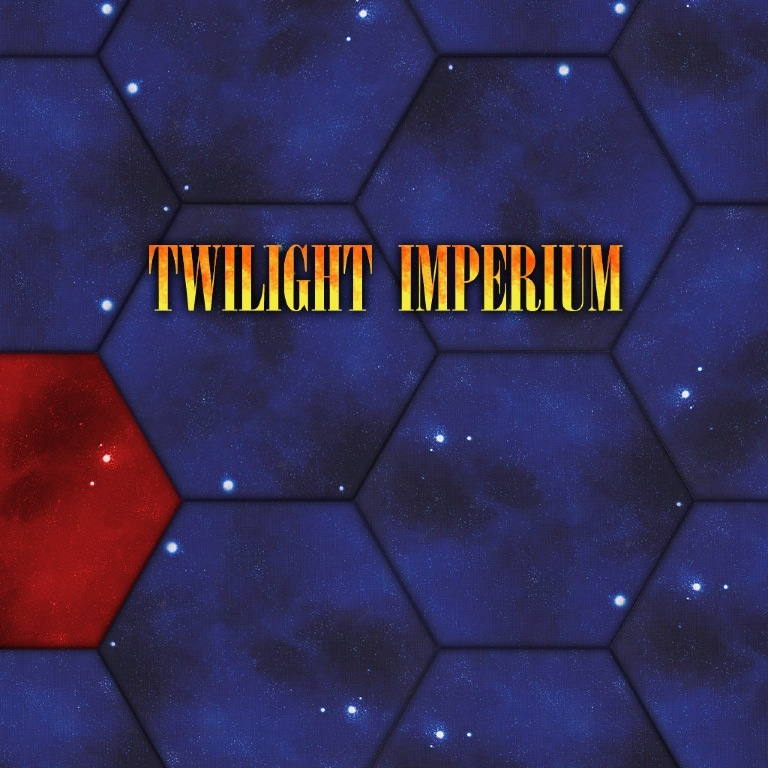
\includegraphics[height=\paperheight, width=\paperwidth]{pic945263}}} % Image background
\centering
\vspace*{10cm}
\par\normalfont\fontsize{1}{1}\sffamily\selectfont
\textbf{Twilight Imperium 3rd Ed.}\\
{\LARGE\textcolor{yellow}{All in One Manual}}\par % Book title
\vspace*{1cm}
{\Huge\textcolor{yellow}{ A Game by Christian T.Petersen}}\par % Author name
\endgroup
%----------------------------------------------------------------------------------------
%	COPYRIGHT PAGE
%----------------------------------------------------------------------------------------

\newpage
~\vfill
\thispagestyle{empty}

%\noindent Copyright \copyright\ 2014 Andrea Hidalgo\\ % Copyright notice

\noindent \textsc{The all in one live Twilight Imperium 3rd edition Manual}\\

% \noindent \textsc{github.com/LaurethTeX/Clustering}\\ % URL



\noindent Originally edited by Max Fuhrmann (bgg:Oigelb) (http://boardgamegeek.com/user/Oigelb).
Many Corrections by bgg:kiminoboku (http://www.boardgamegeek.com/user/kiminoboku).\\ 
This version is also edited by bgg:rafaelolg and bgg:ZaRaZa (http://boardgamegeek.com/user/[rafaelolg, ZaRaZa])\\
\\

\noindent Game Design (all editions): Christian T. Petersen\\
Additional Development (3rd edition): Greg Benage\\
Game Design for the Expansions: Corey Konieczka and Christian T. Petersen\\
Editing: Greg Benage\\
Graphic Design: Brian S. Schomburg, Andrew Navaro and Michael Silsby, Tom Garden and Mark Molnar\\


% License information
\noindent \textit{TWILIGHT IMPERIUM is a trademark of Fantasy Flight Publishing, Inc. Copyright 1997-2011 Fantasy Flight Publishing, Inc. All Rights Reserved. The products, or any parts thereof, may not be reproduced without the publisher's consent.} % Printing/edition date


\begin{table}[!htbp]
\centering
\caption{Versions of this document}
\label{docversions}
\begin{tabular}{|l l l|}
Version & Date        & Comment                                                                          \\
\hline
1.0     & 18.Jan 2012 & First Release                                                                    \\
1.1     & 22.Feb 2012 & Updated to FAQ 2.4                                                               \\
1.2     & 28.Feb 2012 & Corrected FAQ about Flagships and TypeIV Drive and Nano Tech                     \\
1.3     & 24.Apr 2012 & Corrected pagination and player diagram for 7-8 players                          \\
1.4.1   & 26.Aug 2014 & Corrected Front Page                                                             \\
1.4.2   & 06.Dec 2014 & Corrections and houserules from kimioboku                                        \\
1.4.3   & 11.Jul 2015 & Minor Corrections, thx to ZaRaZa                                                 \\
1.4.4   & 21.Jul 2015 & Minor Corrections, thx to ZaRaZa, Kelanen and Arael                              \\
1.4.5   & 17.Oct 2015 & Minor Corrections (FAQ 2.5: Remove systems in 8-player game) and minor graphics. \\
1.5     &  2017       & Move all content to latex . \\
\end{tabular}
\end{table}
%----------------------------------------------------------------------------------------
%	TABLE OF CONTENTS
%----------------------------------------------------------------------------------------

\chapterimage{head1.png} % Table of contents heading image

\pagestyle{empty} % No headers

\tableofcontents % Print the table of contents itself

%\cleardoublepage % Forces the first chapter to start on an odd page so it's on the right

\pagestyle{fancy} % Print headers again

%----------------------------------------------------------------------------------------
%	CHAPTER 1
%----------------------------------------------------------------------------------------

\chapterimage{ti05_preview.jpg} % Chapter heading image
\chapter{Introduction}

\section{The Object of the Game}\index{Objective}
To win a game of TWILIGHT IMPERIUM ("TI"), players seek to accumulate a total of 10 victory points by achieving objectives and carefully choosing helpful strategies. The game ends when one player gains his 10th victory point or immediately after any other game-ending condition applies (see later).

\section{Notations}\index{Notations}

This document has rules that are specific to to optional parts of the game. To make easy to trace and find wich parts you can/want to use this document will use the following notation.

\textbf{Base game} rules will be in the main text.

\begin{SEbox}
Rules and options from \textbf{Shattered Empire Expansion} will be marked with this blue box.
Or just a \SEf{a blue text}.
\end{SEbox}


\begin{STbox}
Rules and Options from the \textbf{Shards of the Throne Expansion} (SoT) will be marked this red box. 
Or just a \STf{red text}
\end{STbox}

\begin{FFGbox}
Online Rules and Options from the FFG-Website will be marked with this green box. 
Or just \FFGf{a green text}.
\end{FFGbox}

\begin{HRbox}
House-Rules and Options (from boardgamegeek.com and ti3wiki.org etc.) with this gray box or just \HRf{a gray text}.
\end{HRbox}



\section{Game Contents and Preparations}\index{Game Contents and Preparations}

\begin{figure}[h]
    \centering
    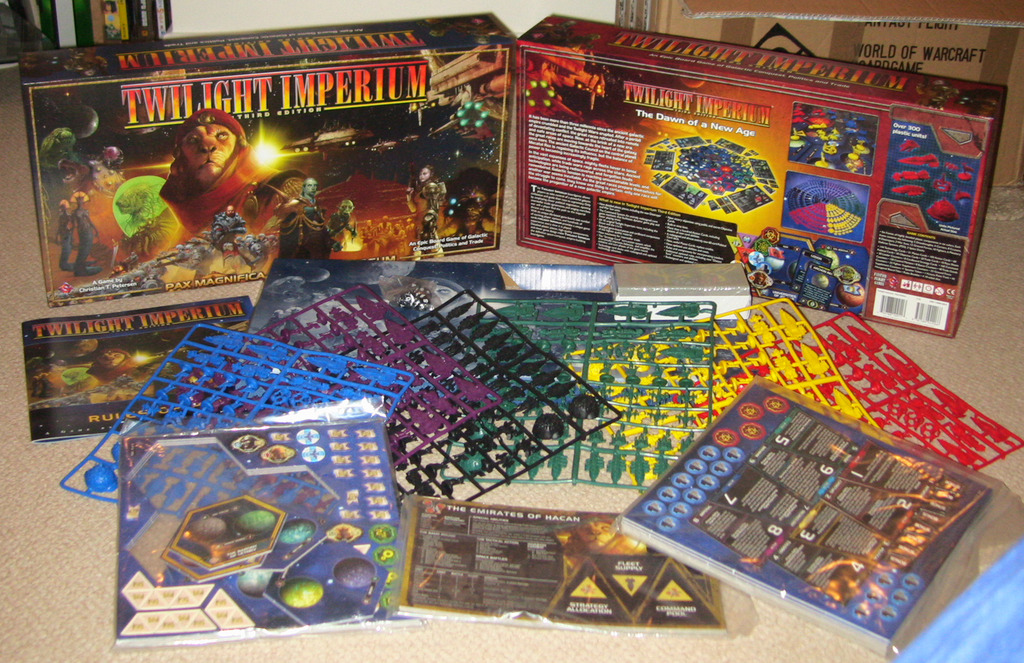
\includegraphics[width=\textwidth]{components.jpg}\\
    \caption{Twilight Imperium 3 straight out of shrinkwrap. image by MattDP@bgg https://boardgamegeek.com/image/222231}
    \label{fig:game_compoments}
\end{figure}


\begin{itemize}
\item 6 \SEf{8 in SE} frames of highly detailed plastic components in 6\SEf{8} colours. Each frame contains the following:
\begin{itemize}
\item 5 Dreadnoughts
\item 4 Carriers
\item 8 Cruisers
\item 8 Destroyers
\item 2 War Suns
\item 12 Ground Forces
\item 10 Fighters
\item 6 Planetary Defense Systems (PDS)
\item 3 Space Docks
\item \STf{1 Flagship}
\item \STf{4 Mechanized Units}
\end{itemize}
\item 256 Technology Cards (32 each in eight decks separated by colour) (24x6 in Base Game, \SEf{28x8 in SE}, \STf{32x8 in SotT}) (\SEf{3 Replaced Techs x 6 in SE})
\item \SEf{34 Race-specific Technologies Cards} (\SEf{14 SE}, \STf{22 SoTT}), (\STf{2 Replaced in SotT})
\item \STf{3 Race-specific Technology Tokens}
\item \STf{17 Flagship Cards}
\item 34 Trade Cards (2 each for 17 races)
\item 51 Leader Counters (3 each for 17 races)
\item 272 Command Counters (16 each for 17 races)
\item 289 Control Markers (17 each for 17 races)
\item \STf{51 Representative Cards (3 each for 17 races)}
\item 17 Race Sheets (10 Basegame, 4 Shattered Empire, 3 Shards of the Throne)
\item 86 Hexagonal Board Tiles (43 from Base Game, 28 from Shattered Empire, 15 Shards of the Throne) 
\item 91 Planet Cards (51 Base Game, 28 SE, 12 SotT)
\item \SEf{16 Facility Cards (8 Colonies, 8 Refineries)}
\item 170 Action Cards (103 Base Game, \SEf{40 Shattered Empire}, \STf{34 SotT}) (7 Replaced Cards (\SEf{5 SE}, \STf{2 SotT}))
\item 110 Political Cards (60 Base Game, 32 Shattered Empire, 19 SotT) (1 Replaced Card)
\item 68 Objective Cards (Secret and Public) (30 Base Game, 28 Shattered Empire, 10 Preliminary SotT)
\item 16 Mercenary Cards
\item 40 Promissory Note Cards
\item 20 Cardboard Strategy Cards (8 Base Game, 8 Shattered Empire, 1 Variant Strategy Card from SE, 3 Variant Strategy Cards from SotT)
\item 8 Bonus Counters
\item 64 Trade Goods Counters (40 Base Game, 12 SE, 12x3 SotT)
\item 51 Fighter Supplement Counters (23x1, 28x3), (23 Base Game, 12 SE, 16 SotT)
\item 51 Ground Force Supplement Counters (23x1, 28x3) (23 Base Game, 12 SE, 16 SotT)
\item \SEf{12 Shock Troop Tokens}
\item \SEf{12 Space Mine Tokens}
\item \SEf{2 Mecatol Custodian Tokens}
\item \SEf{8 Artifact Tokens}
\item \SEf{1 High Alert Token}
\item \SEf{3 Worm Hole Tokens}
\item 66 Domain Counters (44 Base Game, 22 SE,)
\item 15 Space Domain Counters
\item 16 Mercenary Tokens
\item \SEf{8 Unit Reference Cards} (\STf{8 new in SotT})
\item 1 Speaker Token
\item 1 Victory Point Track
\item This rules booklet
\item 4 10-sided dice (note that in TI, the "0" result represents the number "10")
\end{itemize}

\begin{STbox}
\subsubsection{Components of the Scenario “Fall of the Empire”}
\begin{itemize}
\item 1 Race Sheet (the Lazax)
\item 16 Lazax Command Counters
\item 17 Lazax Control Counters
\item 2 Scenario Strategy Cards
\item 34 Agenda Cards
\item 1 Lazax Objective Card
\item 7 Scenario Objective Cards
\item 2 Lazax Trade Agreements
\item 31 Treaty Cards
\item 1 Variant Mecatol Rex Hexagonal Board Tile
\end{itemize}
\end{STbox}

\begin{SEbox}
\subsection{Shattered Empire Components}\index{Shattered Components}
\subsubsection{The Shattered Empire Icon}


\includegraphics[]{se_icon.png}\\

All the cards in this expansion are marked with the \emph{Shattered Empire} symbol on their fronts, to allow you to easily separate them from your base \emph{Twilight Imperium} game.

\subsubsection{Replacement Cards for Base Game}

Several replacement cards for the Twilight Imperium 3rd Edition base game are included in this expansion. Some of these cards have been revised to correct errata, while others have been revised to work better with this expansion. To use the replacement cards, simply remove the original cards from their appropriate decks and replace them with the new versions. The replacement cards are:
\begin{itemize}
\item TECHNOLOGY CARDS
\begin{itemize}
\item 6 Advanced Fighters (1 in each colour)
\item 6 Micro Technology (1 in each colour)
\item 6 Assault Cannon (1 in each colour)
\end{itemize}
\item ACTION CARDS
\begin{itemize}
\item 4 Direct Hit Cards
\item 1 Ruinous Tariff Card
\end{itemize}
\item POLITICAL CARDS
\begin{itemize}
\item 1 Open the Trade Routes Card
\end{itemize}
\end{itemize}
\end{SEbox}

\begin{STbox}
\subsection{The Shard of the Throne Components}\index{Shattered Components}

\subsubsection{The Shard of the Throne Icon }


\includegraphics[]{st_icon.png}

All the cards included in this expansion are marked with the \emph{Shards of the Throne} symbol on their fronts (pictured above), to allow you to easily separate them from your base \emph{Twilight Imperium} game.
\subsubsection{Replacement Cards for Base Game}
\begin{itemize}
\item ACTION CARDS
\begin{itemize}
\item 1 Ghost Ship Card
\item 1 Star of Death Card
\end{itemize}
\item RACE-SPECIFIC TECHNOLOGY CARDS
\begin{itemize}
\item 1 Bioptic Recyclers Card
\item 1 Berserker Genome Card
\end{itemize}
\end{itemize}

\end{STbox}

\section{Component Overview}
We will here summarize the various components of TI, so that you may recognize them while reading these rules.

\subsection{Map Hexes}
Before every game of TI, players will create a unique game board by connecting the provided hexagon map pieces. Each individual piece is called a "system." The systems of TI each represent an area of space, its planets, and/or other elements of interest. Systems that contain an interior yellow outline are \textbf{Home Systems} from which the great races hail. Systems containing an interior red outline are \textbf{Special Systems} (such as Asteroid Fields) governed by special rules.

\begin{SEbox}There are 28 new system tiles in SE, including Ion Storms (a new type of Special System). Hope’s End, the imperial training ground, is also among the new systems. One of the new systems is the Wormhole Nexus (WN), which is easily distinguished by its non-hexagonal shape. Use of this system is optional, and when this rulebook refers to systems, the WN should be excluded unless stated otherwise.
\end{SEbox}

\begin{STbox}
There are 14 new system tiles in SotT, including a Gravity Rift (a new type of Special System) and new Home Systems. A variant version of Mecatol Rex, used only in the Fall of the Empire scenario, is also among the new systems.
\end{STbox}
\subsection{Plastic Game Units}
The detailed plastic pieces of TI (collectively called "units") represent the military personnel, shipyards, defensive systems, and spaceships that players will command. Units not employed on the game board are kept in a player’s reinforcement area.

\subsection{Planet Cards}
Representing the multitude of planets in TI, Planet Cards are used by players to indicate ownership over each individual planet and are "exhausted" (turned face down) when their owner "spends" the planets' resources or influence.

\subsection{Technology Cards}
At the beginning of the game, each player receives an identical Technology Deck (separated by colour) consisting of 24 \SEf{(28 with SE)} \STf{(32 with SotT)} technology advances. Throughout the game, when a player purchases (or otherwise acquires) a technology, the corresponding Technology Card is taken from his deck and placed face-up before him. 
\subsection{ Action Cards}
The Action Cards of TI provide players with a variety of helpful events, manoeuvres, bonuses, and other advantages. Players receive Action Cards throughout the game by a variety of activities.


\subsection{Political Cards}
Often the representatives of the great races must meet in the hallowed halls of the Galactic Council on
Mecatol Rex to debate, deliberate, and enact policy for the custodial imperial charter. When a player executes the primary ability of the Political Strategy Card during the Action Phase (see later), he must draw and resolve the top card of the Political Deck. Each Political Card contains an \textbf{agenda} that all players must vote upon. The effects of an agenda can range from a minor formality, to a major change in the very structure of the game.

\subsection{Objective Cards (Public and Secret)}
In order to win TI, players need to accumulate 10 victory points. The primary way for players to receive such is by qualifying for the requirements of an Objective Card. The victory points provided by Public Objective Cards are attainable by all players, whereas those from Secret Objective Cards are individual to each player.
\begin{SEbox}
    
The new sets of Stage I and Stage II Public Objectives can optionally be used instead of the original Objective deck. These cards tend to focus more on military conflict than the original set. Also provided are 3 new Secret Objectives, to be mixed in with the original set.
Finally, Special Objectives have been included for use with two new optional rules: Artifacts (detailed on page 65) and the Voice of the Council option (detailed on page 68).
\end{SEbox}
\begin{STbox}
Preliminary Objective Cards optionally start players with easier objectives worth 1 victory point each. Also provided are Scenario Objective Cards, only used in the Fall of the Empire scenario (including a special Lazax Objective Card).
\end{STbox}
\begin{STbox}
    
\subsubsection{The Secret Objective Deck}
Some cards and rules in this expansion refer to the Secret Objective deck. This deck consists of any Secret Objective not in play. Instead of placing unused Secret Objective cards in the box, simply place them in the play area. When a player fulfils a Secret Objective card, it is removed from the game (and not shuffled back into this deck).
\end{STbox}

\subsection{Trade Cards}
Each race has two Trade Contract cards which they can use to form trade agreements with other players. Each Trade Card has a numerical trade value which varies from race to race.

\subsection{Strategy Cards}
Each of the eight cardboard Strategy Cards represents a powerful short-term strategy. During the Strategy Phase of each game round, each player will select one Strategy Card and must later use its primary ability. Each Strategy Card also enables an important secondary ability that other players may execute after the primary ability is resolved.
\begin{SEbox}
    
SE  features a new set of eight variant Strategy Cards, with a white background, that favours different strategies than the original set. In addition, there is a High Alert token for use with the new Warfare II Strategy Card. The variant Imperial Strategy Card, with a black background, may optionally be used with the original set of Strategy Cards.
\end{SEbox}
\begin{STbox}
SotT  features variant Political, Assembly, and Trade Strategy Cards. Two Strategy Cards only used for the “Fall of the Empire” scenario are also included (Civilization and Industry, s. page 76).
\end{STbox}

\subsection{Bonus Counters}
After all players have selected a Strategy Card during the Strategy Phase, there will (in a six-player game) be two Strategy Cards remaining in the common play area. Before the Strategy Phase ends, the two remaining Strategy Cards both receive a Bonus Counter that is placed on top of the Strategy Card itself. A player that later selects such a Strategy Card will be able to use the Bonus Counter to receive an additional Command Counter or Trade Good.


\subsection{Command Counters}
The Command Counter in TI is the abstract but integral resource representing the domestic mandate,
budget, organization, logistics and preparedness of your race. When a player receives a Command Counter from his reinforcements, he must place it in either the Fleet Supply area, Strategy Allocation area, or Command Pool area on his Race Sheet. In order to execute tactical actions (such as moving, building, or initiating combat on the board), take advantage of the secondary abilities of Strategy Cards, or manage his fleets, a player must wisely allocate and spend Command Counters.

\subsection{Control Markers}
At the beginning of the game, each player is provided with a generous number of flag-shaped Control Markers, each bearing the insignia of that player's race. The Control Markers are used to represent a race wherever appropriate, such as on the Victory Point Track, on successfully achieved Objective Cards, and (most often) to indicate ownership of planets.

\subsection{Trade Good Counters}
These counters represent the wealth and rewards of interstellar commerce. They are primarily obtained by active trade agreements while the Trade Strategy Card is being executed. A player's Trade Goods can be used as a direct substitute for either resources or influence, and are frequently used as currency among players to pay for bribes or other considerations.

\subsection{Victory Point Track}
The Victory Point Track is used to indicate each player's accumulation of victory points. Note that the main side of the Victory Point Track has spaces numbered from 0 to 10, whereas the reverse side is numbered 0 to 14. The reverse side is be used with the optional rule “The Long War” found on page 57.

\subsection{Speaker (First Player) Token}
This token is claimed each round by the player who selects the Initiative Strategy Card during the Strategy Phase. The player who controls the Speaker Token always chooses the first Strategy Card during the next Strategy Phase.

\subsection{Ground Force and Fighter Unit Supplement Tokens}
The Ground Force and the Fighter units are the only units in the game that players may purchase unlimited quantities of. All other unit types are limited to the figures provided with the game. The Fighter and Ground Force supplement tokens represent the extra Fighter and Ground Force units that players may add to their forces.

\subsection{Race Sheets}
Enclosed in your game, you will find 10 (\SEf{14 with SE}, \STf{17 with SotT}) large cardboard sheets, each representing one of the great races of the TI universe. After selecting a race to play, each player receives the corresponding Race Sheet, which provides each player with specific information for his race as well as helpful game information tables. The Race Sheet is also used for keeping track of a player’s active Command Counters and Trade Goods.
\begin{STbox}
A race sheet for the Lazax is also included in SotT. The Lazax race is only used in the “Fall of the Empire” scenario (see page 76). Cards and Markers are also provided for this race.
\end{STbox}
\begin{SEbox}    
\subsection{Race-Specific Technologies}

Each of the 17 races now has one Race-Specific Technology. These optional Technology cards may only be acquired by the appropriate race (see page 64). \STf{In SotT there is a second race-specific Technology per Race included.}

\subsection{Facility Cards}
These cards represent refineries and colonies that players may build on a planet to increase the planet’s resources or influence value. See page 67 for details.

\subsection{Unit Reference Cards}
The unit reference cards provide players with an image of each unit type and its game stats.

\subsection{Shock Troop Tokens}
Shock Troops represent battle-hardened, veteran Ground Forces. These special Ground Forces are much more powerful and have special rules governing them (found on page 65).

\subsection{Space Mine Tokens}
With the new Space Mines option, Cruisers have the ability to deploy space mines. Ships moving into a system that contains space mines could be destroyed before combat. See details on page 66.

\subsection{Mecatol Rex Custodian Tokens}
These tokens represent guardians of Mecatol Rex. Their optional use is described on page 68.

\subsection{Artifact Tokens and Objective Cards}
These tokens represent four ancient relics of power that are hidden somewhere through out the galaxy. Each Artifact also has a corresponding Special Objective card worth 1 Victory Point to its controller., See details on page 65.

\subsection{Wormhole Tokens}
Special Wormhole tokens have been included for use in optional map setups.

\end{SEbox}

\begin{STbox}
\subsection{Agenda Cards}
These cards replace the Political Card deck when playing the “Fall of the Empire” scenario.

\subsection{Flagship Cards}
Each of the 17 races now has the ability to build its own Flagship, a powerful warship with unique race-specific abilities. These optional ships may only be built by the appropriate race (see page 70).

\subsection{Mercenary Cards}
These cards represent Mercenaries that players may hire using the new Trade III Strategy (s. page 72).

\subsection{Promissory Note Cards}
Players can now offer Promissory Notes in the Galactic Council. These new cards are used with the new Political II and Assembly II Strategy Cards (see page 74).

\subsection{Representative Cards}
Each of  the races has 3 Representatives that players may choose from to send to the Galactic Council. These optional cards are used with the new Political II and Assembly II Strategy Cards (see page 13).

\subsection{Treaty Cards}
These cards are only used in the “Fall of the Empire” scenario. Players can make alliances with each other using these cards.

\subsection{Space Domain Counters}
These new counters are used with the Final Frontier option. See page 70 for more information).

\subsection{Mercenary Tokens }
These tokens mark the locations of Mercenaries (a new type of unit) on the board. They are double-sided to display whether the Mercenary is in space or on a planet. The appropriate battle value for each Mercenary is also displayed on each side.

\subsection{Race-specific Technology Tokens }
Special Tokens have been included for use with the Ghosts of Creuss’ and the Embers of Muaat’s special abilities.

\end{STbox}
\chapterimage{rexbanner.jpg}
\chapter{Setup}\index{Setup}
\begin{figure}[h!]
    \centering
    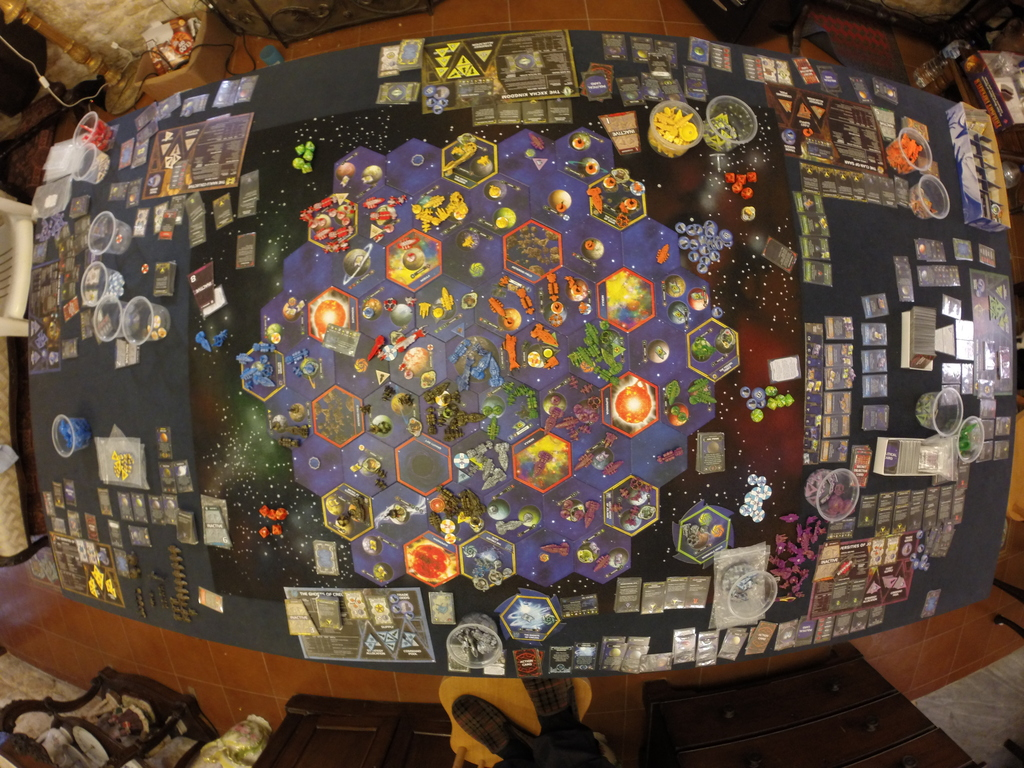
\includegraphics[width=\textwidth]{gametable.jpg}\\
    \caption{8 player game. Photo by tintii@bgg https://boardgamegeek.com/image/2355207}
    \label{fig:game_table}
\end{figure}

\section{Number of Players}
These rules are written assuming that you will be playing TI with 6 players. TI plays just as well with
fewer players, and rules for playing with 3-8 players are provided on page 53 of this rules set.


\section{Setup and Play Area Organization}

\begin{figure}[!h!]
    \centering
    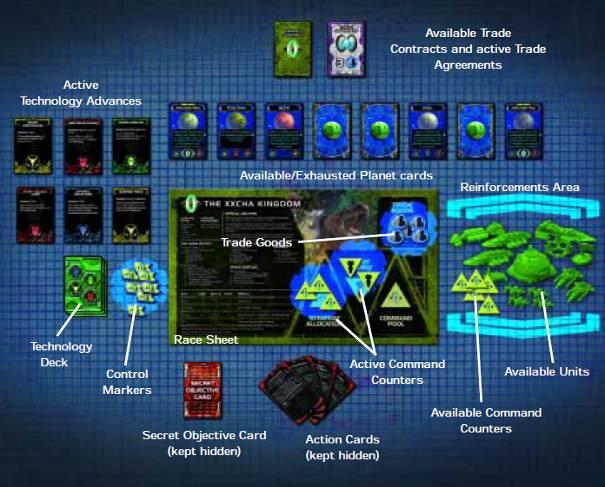
\includegraphics[width=\textwidth]{playarea.jpg}\\
    \caption{Suggested Player Area}
    \label{fig:play area}
\end{figure}

\begin{figure}[!h!]
    \centering
    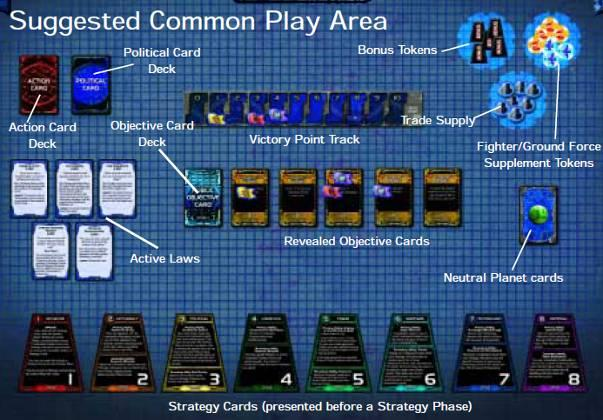
\includegraphics[width=\textwidth]{commonplayarea.jpg}
    \caption{Suggested Common Play Area}
    \label{fig:play area}
\end{figure}

Before you start playing, follow the steps below:
\begin{enumerate}
\item Separate the 10 Home Systems from the other hexagonal game-board pieces. Randomize the Home Systems face down and allow every player to draw one at random. This process determines which race a player will control throughout the game. All players then take the Race Sheet, Control Markers, Trade Cards, and Command Counters corresponding to their race.
\item Each player selects one of the six available colours and takes the plastic units and Technology Deck corresponding to that colour.
\item Find an area of the table that is convenient for all players to reach. Designate this space the "common play area." Then shuffle the Action Card deck and the Political Card deck and place them separately in the common play area. Also place the Fighter and Ground Force Supplement Counters in the common play area.
\item Each player takes the individual Planet Cards corresponding to the planets of his Home System and places these face up in his play area. Place the remaining Planet Cards, representing the neutral planets at the start of the game, in the common play area.

\item Place all the Trade Goods Counters in a single pile (the "Trade Supply") in the common play area.
\item Now place the 8 Strategy Cards side-by-side in numerical order with their "active" side up, prominently in the common play area.
\item Create the Objective Deck, by following the directions in the "Preparing the Objective Cards" sidebar. Do not forget to place the unused Secret and Public Objective Cards back in the box, while allowing no players to look at them.
\item Now place the Victory Point Track in the common play area and place one Control Marker for each player in the space marked "0."
\item Players must now create the game board (or “galaxy”). Please read and carry out the instructions for doing so in the "Setting up the Galaxy" sidebar on page 15 before proceeding.
\item After the galaxy has been created, all players place their "setup units" (as indicated by their Race Sheets) on their Home Systems. If a Home System contains several planets, any Space Dock, Ground Forces, and PDS may be placed among them according to the player’s wishes.
\item All players then find and place their "Starting Technology" cards face up in their respective play areas. All players now take their starting Command Counters from their reinforcements, placing them on their Race Sheets as follows: \textbf{2 Command Counters in the Strategy Allocation area, 3 Command Counters in the Command Pool area, and 3 Command Counters in the Fleet Supply area (with the "Fleet" side up)}.
\end{enumerate}


\subsection{Reinforcements}
Every player maintains a “reinforcement” area consisting of his unused plastic units and Command Counters. Whenever a player builds a unit, it is taken from his available reinforcements and thereafter placed on the board. (An exception to this is the Fighter and Ground Force Supplement counter, see later). Whenever a player receives a new Command Counter, it is taken from his available reinforcements and placed in one of the three appropriate boxes on his Race Sheet (Command Pool, Fleet Supply, or Strategy Allocation).

\subsection{Preparing the Objective Cards}
Before the game begins, the Secret Objective Cards must be distributed and the Public Objective Deck properly prepared. First separate all the Objective Cards into the three different types: Secret Objectives, Public “Stage I” Objectives, and Public “Stage II” Objectives. Then proceed to the following:

\begin{enumerate}
\item Shuffle the 10 Secret Objective Cards and deal a random card face down to every player. All players should read their Secret Objective Card and then place the card face down in their play area. A player is never allowed, for whatever reason, to show an opponent his Secret Objective Card. Place the remaining Secret Objective Cards back in the box, allowing no player to look at them.
\item Now take the 10 Stage II Public Objective Cards and remove the “Game Over” card. Shuffle the remaining 9 Stage II cards and draw 3 random cards (at all times keeping them hidden from all players). After drawing the 3 random cards, take the “Game Over” card and shuffle it with the 3 randomly-chosen cards. You should now have 4 randomized Stage II Public Objective Cards, one of which is the “Game Over” card. Place these 4 cards face down in a stack in the common play area. Place the remaining Stage II cards back in the box, allowing no player to look at them.
\item Then shuffle the 10 Stage I Public Objective Cards and draw 6 random cards. Place the 6 cards on top of the 4 Stage II cards, now forming a single deck of 10 Public Objective Cards in the common play area. This deck always consists of 6 random “Stage I” cards on top of 4 random “Stage II” cards (one of which is the “Game Over” card). This deck is the “Public Objective Deck.”
\end{enumerate}

\begin{STbox}   
     It is important that the unused Objective Cards (Secret, Public Stage I \& II) are placed back in the box so they remain hidden from players both before and during the game. Otherwise, experienced players would be able to deduce which objectives are in play before they are revealed.

\end{STbox} 

\emph{You are now ready to start the game.}



\chapterimage{twilight-imperium.jpg}
\chapter{Rules}\index{Rules}

\section{Objective of the Game}\index{Objective}
To win a game of TWILIGHT IMPERIUM ("TI"), players seek to accumulate a total of 10 victory points by achieving objectives and carefully choosing helpful strategies. The game ends when one player gains his 10th victory point or immediately after any other game-ending condition applies (see later).

\section{Creating the Galaxy}

\begin{figure}[!h!]
    \centering
    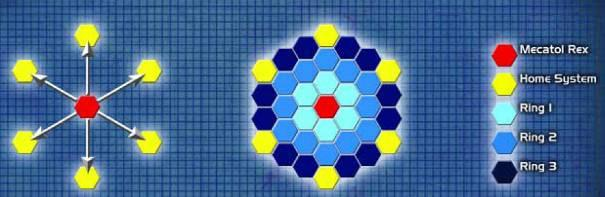
\includegraphics[width=\textwidth]{creating_galaxy.jpg}
    \caption{Galaxy creation schematics}
    \label{fig:galaxycreation}
\end{figure}
TI uses a unique game board consisting of multiple hexagon pieces (“systems”) that are brought together in a unique combination at the beginning of every game. Players build the galaxy by following these steps:

\begin{enumerate}
\item After all players have drawn their Home Systems, find the Mecatol Rex system and place it in the middle of the table. Then randomly determine one player to be “first player. Give the “Speaker“-Token to the first player. He then shuffles the remaining 32 systems, \emph{randomly removes two systems} (by placing them back in the box without looking at them), and deals five systems, face down, to every player. Players may look at their dealt systems but should not show them to the other players.
\item The first player now selects one of the sides of Mecatol Rex, and drags his Home System about two feet towards himself in a straight line away from the chosen side (see diagram). Then the player to his left does the same, etc., until all players have chosen a side and placed their Home Systems on the table (note that the sixth player must chose the last remaining side of Mecatol Rex). Players should now shift their seating around the table to best accommodate their Home System placement.
\item Then players, in clockwise order, starting with the first player, begin creating the galaxy by placing, one at a time, a single system face up adjacent to the Mecatol Rex system. After the first ring around Mecatol is completed, players continue to place systems in the second ring until that is completed, and then finally proceed to the third ring.
\end{enumerate}

When all the systems are placed, the galaxy is finally created. The following rules apply to placing systems:

\begin{itemize}
\item A system cannot be placed in the second ring before the first ring surrounding Mecatol Rex has been completed. Likewise, a tile cannot be placed in the third ring before the second ring is completed (see diagram).
\item As soon as the correct placement for your Home System becomes available, connect your Home System to the galaxy at its fixed spot (which is exactly 3 systems out from the chosen side of Mecatol Rex, see diagram). Connecting your Home System is automatic and does not cost you a placement “turn.”
\item You may not place a Special System (with an inner red border) adjacent to another Special System, unless you have no other option.
\item The order of placement switches counter clockwise after all players have placed a round of tiles and yet again clockwise after that, etc. This in effect will make the player, who placed the last system, place the first system in the next round (thus actually placing two systems in a row). Example of turn order: P1, P2, P3, P4, P5, P6, P6, P5, P4, P3, P2, P1, P1, P2…
\item If you placed a system that did not contain a planet during your last placement, you must, if able, place a system that \emph{does} contain a planet during your next placement. If you are unable to do so, you must reveal your remaining systems to the other players to prove this. Then place one of your available systems.
\end{itemize}

When creating the board, the actual shape of the galaxy and the position of Home Systems will differ depending on the number of players. If you are playing a game with less than six players, please consult the optional rules on page 53 of this rules booklet.

\begin{SEbox}
    \subsection{Game Setup with the New Systems from the Expansion Shattered Empire}
    Due to the addition of many new systems, players will need to remove more random systems before setting up the galaxy than specified in the base game.

The first player should place these systems back in the box during setup without looking at them.

Remove the following systems instead of the systems specified on page 53 of the original rulebook:
\begin{itemize}
\item 3 Players: Remove 7 empty, 6 Special, and 18 Regular Systems (with planets).
\item 4 Players: Remove 4 empty, 5 Special, and 14 Regular Systems (with planets).
\item 5 Players: Remove 4 empty, 5 Special, 14 Regular Systems (with planets), and 1 random system.
\item 6 Players: Remove 4 empty, 5 Special, 14 Regular Systems (with planets), and 2 random systems.
\end{itemize}
\subsection{Larger Galaxy Games}
With five or six players, players may wish to set up an additional outer ring. To do this, fewer tiles are removed during setup.
\begin{itemize}
\item 5 Players: Deal out every tile, so that each player has 11 tiles. Then create the galaxy as normal. (Unlike the standard 5-player setup described on page 32 of the original rules, no random system is placed adjacent to Mecatol Rex.)
\item 6 Players: Remove 1 random hex and then deal out the rest, so that each player will have 9 tiles.
\end{itemize}

Then create the galaxy as described on page 8 of the original rulebook. However, in step 3 of “Creating the Galaxy,” continue placing systems until there are 4, rather than just 3, rings around Mecatol Rex.
\end{SEbox}


\begin{STbox}
\subsection{Game Setup with the New Systems from both Expansions}

Due to the addition of many new systems, as well as the systems introduced in Shattered Empire, players now have more options when setting up the galaxy. Instead of removing the systems specified on page 53 of the original rulebook, players create three piles of systems; one pile of Special Systems (all systems with red borders), one pile of empty systems (all systems with no planets), and one pile of Regular Systems (all remaining non-Home Systems). Without looking at the tiles, players deal a number of random systems into a galaxy pile and shuffle it. All remaining tiles are returned to the game box without looking at them. Players then use the systems in this galaxy pile to create the galaxy (following all normal setup rules).

\begin{itemize}
\item 3 Players: Shuffle together 3 Special, 5 empty, and 16 Regular Systems.
\item 4 Players: Shuffle together 4 Special, 8 empty, and 20 Regular Systems.
\item 5 Players: Shuffle together 4 Special, 8 empty, and 20 Regular Systems. Randomly remove 1.
\item 6 Players: Shuffle together 4 Special, 8 empty, and 20 Regular Systems. Randomly remove 2.
\SEf{
\item *7 Players: Shuffle together 9 Special, 12 empty, and 34 Regular Systems, randomly remove 2
\item *8 Players: Shuffle together 9 Special, 12 empty, and 34 Regular Systems, randomly remove 3
\item *5 Players (Larger Galaxy): Shuffle together 9 Special, 12 empty, and 34 Regular Systems.
\item *6 Players (Larger Galaxy): Shuffle together 9 Special, 12 empty, and 34 Regular Systems. Randomly remove 1.\\
\item *Requires the Shattered Empire expansion.}
\end{itemize}
\end{STbox}

\section{The Game Round}
After you have finished setting up the game, players will begin playing the game by starting with the
\emph{Strategy} Phase of the first game round. TWILIGHT IMPERIUM is played over a consecutive number of game rounds with each round consisting of the following phases:

\begin{itemize}
    \item The Strategy Phase
    \item The Action Phase
    \item The Status Phase
\end{itemize}

After every Status Phase, if no player has yet declared victory, simply begin another game round starting with another Strategy Phase, etc. In this way the game continues, repeating the three phases above, until a player has achieved 10 victory points or until another game-ending condition is met.

Victory points are generally claimed during the Status Phase as players fulfil the requirements printed on the Public and Secret Objective Cards. In order to meet these various objectives, players must seek to expand their empires, forge alliances with other races, negotiate for the best outcome during the Galactic Council, and choose the optimal Strategy Cards during the Strategy Phase.


\subsection{ Strategy Phase}
During every Strategy Phase, each player must choose one available Strategy Card from the common play area (The chosen Strategy Card grants its player a special ability during the upcoming Action Phase.) At the beginning of every Strategy Phase, there are 8 possible Strategy Cards (or "strategies") that players may choose from. These are: Warfare, Political, Trade, Initiative, Imperial, Logistics, Diplomacy, or Technology.

Not only does the Strategy Card provide an important ability, but it also determines the \emph{order of play} (as indicated by its number; see the text box on page 20 for more information on the order of play).
At the beginning of every Strategy Phase, the player who controls the Speaker Token (the "Speaker") may choose the first Strategy Card from the common play area.

When selecting a Strategy Card, a player simply chooses and takes an available Strategy Card from the common play area and places it before him (with the "active" side facing up).

That card is now no longer available for selection by the other players.

After the Speaker has picked his Strategy Card, the other players, in clockwise order from the Speaker, each select one of the remaining Strategy Cards. In this way every player will pick an available Strategy Card before the Action Phase begins. Note that being farther clockwise from the Speaker gives a player an increasingly limited choice of Strategy Cards (i.e., the player to the immediate right of the Speaker will only have three cards to choose from).

After all players have selected a Strategy Card, there will be two cards remaining in the common play area. The Speaker places a \emph{Bonus Counter} on the two remaining unchosen Strategy Cards.

In this way, should a Strategy Card not be picked for several consecutive rounds, multiple Bonus Counters will accumulate on it.
The presence of Bonus Counters makes a Strategy Card more attractive in subsequent rounds.

When a player selects a Strategy Card that contains one or more Bonus Counters, that player may immediately exchange each Bonus Counter for either a Trade Good or a Command Counter (either of which is immediately placed on the player's Race Sheet).

After all players have chosen their Strategy Cards and the Bonus Counters have been placed on the remaining cards, the Strategy Phase ends and the game proceeds to the Action Phase.

Note that the last player to claim the Speaker Token will keep the Speaker Token until another player selects the Initiative card during a future Strategy Phase.

\subsection{Action Phase} % (fold)
\label{sub:action_phase}

The Action Phase forms the heart of TI. It is during the Action Phase that players will execute the special abilities of their Strategy Cards, produce new units at their Space Docks, conquer new planets, and move their fleets into battle.

rn order would be the player who selected the Diplomacy Strategy.


The Action Phase is resolved over a number of \emph{player turns} in which each player may take a \emph{single action}. Each player turn is taken in the order of play (see text box on page 21), with players one after the other taking one action to complete their turn. After the last player in the order of play has taken his turn, play returns once more to the first player in the order of play who may take an action, followed by the second player, and so on. In this way, players keep taking one action at a time, following the order of play, until all players have passed and the Action Phase ends.

\subsubsection{Order of Play}
Each Strategy Card has an Initiative Number printed near its top. This number represents what place in the order of play its owner will be. Thus, the player who has the Initiative Strategy card is always first, followed by the player who controls the Diplomacy Strategy card, etc. The order of play, as dictated by the Strategy Cards, is as follows:
\begin{enumerate}
    \item Initiative Strategy
    \item Diplomacy Strategy
    \item Political Strategy
    \item Logistics Strategy
    \item Trade Strategy
    \item Warfare Strategy
    \item Technology Strategy
    \item Imperial Strategy
\end{enumerate}

When the turn order advances to an unchosen Strategy Card in the common play area, simply skip it and proceed to the next number. If, for example, no player picked the Initiative Strategy card during the Strategy Phase, the first player in the tu

A player that is currently in the process of taking his turn (i.e., action) is called the \emph{active player}. When it is a player's turn to take an action, he must execute one of the following:
\begin{itemize}
\item Strategic Action
\item Tactical Action
\item Transfer Action
\item Pass 
\end{itemize}

% subsubsection the_player_action (end)

\subsection{Strategic Action} % (fold)
\label{sub:strategic_action}
A player must, at some point during the Action Phase, execute a Strategic Action (except for the player holding the Initiative Strategy Card, who has no Strategic Action).

When a player chooses to take his Strategic Action, he first reads and then resolves the \emph{Primary Ability} as printed on his Strategy Card. After the active player has finished resolving the Primary Ability, the other players, in \emph{clockwise order from the active player}, may each spend one Command Counter from their Strategy Allocation area on their Race sheet to execute the \emph{Secondary Ability} of the current Strategy Card.

\begin{STbox}
    \emph{Special Exception}: Players do not have to spend a Command Counter from their Strategy Allocation area when executing the Secondary Ability of the Logistics Strategy Card.
\end{STbox}

The active player \emph{may never} execute the Secondary Ability of his own Strategy Card.
After all players have completed (or passed on) the Secondary Ability, the active player's Strategy Card is flipped over onto its "Inactive" side and the player action is over.
A player may only take one Strategic Action per round. Likewise, a player may only execute any given Secondary Ability once (but a player may, if he has a sufficient number of Command Counters in his Strategy Allocation area, participate in the Secondary Ability of several Strategy Cards).
The initiative number on each Strategy Card only determines the order of play. Players may execute
their Strategic Action at a time of their choosing, regardless of its initiative number.  It is likely, for example, that the player holding the Trade Strategy will take his Strategic Action before the player holding the Logistics Strategy, even if the Logistics Strategy has a lower initiative number. Details for each specific Strategy Card can be found on page 88.  

\subsection{Tactical Action} % (fold)
\label{sub:tactical_action}

The Tactical Action is the primary function for engagement on the game board. It is during a Tactical
Actions that you will move your fleets on the board, engage in space battles, transport your Ground Forces to new planets, build new units, etc. 
The process of taking a Tactical Action always follows the "Activation Sequence" below:


\emph{The Activation Sequence}
\begin{enumerate}
\item Activate a system
\item Move ships into the system
\item PDS fire
\item Space Battle
\item Planetary Landings
\item Invasion Combat
\item Produce Units
\end{enumerate}

Except for the first step (the activation itself), each individual step of the Activation Sequence is only resolved if the condition for its resolution applies or is initiated by the active player. 

A player, for example, may activate a system to produce new units there during step 7, but does not necessarily have to move any ships into the system during step 2. Or, a player may activate a system and move ships into the system, but if the system contains no enemy ships, there is no Space Battle during step 4, etc.
On the other hand, step 2 through 7 cannot be executed unless preceded by the initial activation.

If a player has no Command Counters left in his Command Pool, he cannot take a Tactical action, and therefore not move ships, fight battles, produce units, etc.
\begin{FFGbox}
    \emph{“Friendly“ and “Enemy“}

When the cards and rules of TI refer to a “friendly” unit or planet, it refers to a unit or planet belonging to you (i.e., a single player). Although you may have an alliance or be personally friendly with another player, for the purposes of TI rules, only your own units and planets are “friendly”.

When the rules refer to an “enemy” planet or unit, it refers to any unit or planet not controlled by you (i.e., controlled by any other player). Even though you may have an alliance with another player, and even though you may consider the other players your personal friends, for the purposes of TI rules, the units and planets of other players are considered “enemy.”

\end{FFGbox}

\subsubsection{Activation Sequence in Detail}
Below, each step in the Activation Sequence is described in detail. Rules for how to resolve Space Battles and Invasion Combat can be found on pages 27 through 30.

\begin{description}
\item [1 - Activate a System] Take an available Command Counter from your Command Pool and use it to activate a system by placing the Command Counter directly on a system (place the counter face-up so that your race's insignia is showing). You cannot activate a system if one of your Command Counters has already been placed in the system (by a prior activation or by other means). You can, however, activate a system that contains one (or more) Command Counters belonging to other races (you may ignore their presence). A system that contains a player's Command Counter is considered to have been \emph{activated} by that player.  

\emph{In summary}: When the TI rules and cards refer to an "activated" system, this means a system that contains a Command Counter of the player in question. 
As a general rule, for purposes of activation and movement, a player can ignore the presence of Command Counters on the board belonging to other players.

This means, for example, that every race can activate a specific system. In such a case, that system would contain a Command Counter from each race and would be considered “activated” by all players.  Although the Command Counters on the board belonging to other players do not limit where you may activate a system, it can be helpful to study which systems an opponent has activated, since those system cannot be activated again by that player this round, nor can his ships in his activated systems move. 

\item [2 -  Move Ships into System] 
After you have activated a system, you may move friendly ships (within movement range) into the activated system. \emph{Only movement into the activated system is allowed.}

The rules for moving ships during a Tactical Action are as follows:
\begin{itemize}
    \item Every ship (except for Fighter units, which move with Carriers or War Suns) has a movement value found on the unit table located on every player's Race Sheet. A movement of "1" indicates that a ship can move from its current system into an adjacent system. A movement of 2 indicates that the ship may move up to two systems from its current system, etc.
    \item A Carrier/War Sun may pick up Ground Force and PDS units at any stage during the movement step (before, during, and even in the activated system itself). Ground Force and PDS units aboard a Carrier, however, cannot be "dropped off" by the Carrier until the Planetary Landing step of the Activation Sequence. \emph{If the last Ground Force unit on a planet is picked up by a Carrier, the owner of the planet must place a Control Marker on the planet to indicate that he controls it}. There are some exceptions to this rule (See P.45 for Ground Force and P.46 for Carrier).
    
    \item A ship is never allowed to move through a system occupied by enemy ships (except Fighters). The only way to enter a system that contains enemy ships is to activate that system itself.

    \item A ship may not move if it is located in a system that already has been activated by the active player (i.e., contains a friendly Command Counter placed prior to the current activation). It therefore follows that, once a ship has moved into an activated system, the very Command Counter used for the activation will prevent the ship from moving again during the same round. Ships \emph{are allowed to move through} systems containing friendly Command Counters.
\end{itemize}
Certain effects by Strategy or Action Cards can remove Command Counters from the board, allowing systems to be activated again by the same player (and allowing any friendly units in such a system to move again, etc).

\emph{In summary}: Only ships that can actually enter the activated system may move. 
Ships that are out of movement range, that need to pass through a system containing enemy units, or are in a system already activated, may not move. Remember, any ship moving must always end its movement in the system that was just activated. See the detailed graphical example of a Tactical activation and movement on page 24.


\item[3 - PDS Fire]
After the active player has finished moving his ships into the activated system, enemy PDS in range may fire at the active player's fleet. For every "hit," the activating player must remove a casualty from the fleet (note that Dreadnoughts and War Suns can take one "Damage" before they are destroyed, see page 52). After enemy PDS units have fired, any PDS in range owned by the active player may then fire at enemy ships in the activated system. For more details on PDS units, see page 48.

\item[4 - Space Battles]
First determine whether a Space Battle will occur in the activated system.
If the active player has moved one or more ships into a system that contains ships controlled by an opponent (even a Fighter) a Space Battle \emph{must} be initiated between the two players.

A Space Battle will continue until only one player has ships remaining in the system. If a Space Battle is initiated, the active player is the \emph{Attacker} and the player whose ships were in the system before activation is the \emph{Defender}.  For complete rules of how to resolve a Space Battle, please see the “Space Battles” section on page 27]

\item [5 - Planetary Landings] 
After any Space Battles are completed, the active player may now commence Planetary Landings by landing Ground Force and PDS units from his Carriers onto planets in the activated system.

If a system contains multiple planets, the active player may split any landing forces between them in any way he sees fit, but may not change his mind once the Invasion Combat step begins. There are three types of Planetary Landings:
\begin{description}
    \item [Friendly Landing] A player lands units on a planet already under his control. Simply add the new units to the ones already there, if any.

    \item [Neutral Landing] A player lands units on a neutral planet (i.e., a planet controlled by no other player). After landing at least one Ground Force unit on the neutral planet, the active player takes the corresponding Planet Card from the Planet Deck and places it exhausted in his play area. Note that only a Ground Force unit can take over a planet. If a PDS unit lands alone on a neutral or enemy planet, it is immediately destroyed.

    \item[Hostile Landing (also called an "Invasion")] A player lands units on a planet containing one or more of an enemy player’s Ground Force units. This will result in an Invasion Combat during the Invasion Combat step.
\end{description}

If a player lands units on a planet that is controlled by an opponent, but does not contain any enemy Ground Forces, the planet falls without resistance. The invader simply removes the opponent’s Control Marker and takes the corresponding Planet Card from the opponent, placing it exhausted into his play area.

\item [6 Invasion Combat] After planetary landings, should any planet contain Ground Forces of two different players, that planet must now engage in Invasion Combat.  If a system has several planets engaged in Invasion Combat, the battles are resolved one-at-a-time in the order decided by the active player.

\emph{Landing PDS units with an Invasion:} The invading player is allowed to land PDS units with his Ground Forces during the Planetary Landings step. Such PDS units do not participate in Invasion Combat, nor can they be taken as a combat casualty. If the last invading Ground Force unit is destroyed during Invasion Combat, all invading PDS are immediately destroyed with no further effect. 
Details for how to resolve Invasion Combat are found in the “Invasion Combat” section on page 30.

\item[7 - Produce Units]
As the final step of a Tactical Action, the active player may produce new units at one or more friendly Space Docks in the activated system. During this step, it is also possible for the active player to produce a new Space Dock unit on an eligible planet in the activated system (provided that the planet has been under the player’s control for the entire round). See more information on how to produce units under the Space Dock on page 44 concluding a Tactical Action.

After resolving the steps of the Activation Sequence (Activate a system, Movement, PDS fire, Space Battles, Planetary Landings, Invasion Combat, and Production), the Tactical Action is over and the opportunity to take an action proceeds to the next player in the order of play.

\end{description}
\begin{FFGbox}
    \subsubsection{Definition of a Fleet}
    For the purposes of the TI rules and cards, a fleet is defined as all spaceships (Fighters, Cruisers, Carriers, Dreadnoughts, Destroyers, and War Sun units) controlled by one player in one system at any given time.
\end{FFGbox}


\subsection{Transfer Action} % (fold)
\label{sub:transfer_action}
The Transfer Action is a simple reorganization of units that cannot be effectively handled by the Tactical Action. The Transfer Action simultaneously activates two \emph{adjacent systems that only contain units belonging to the active player} and allows units in either system to simultaneously move between the two systems. In addition to this movement, the active player may also produce units in one of the two systems if a Space Dock is present in either. The process of taking a Transfer Action always follows the steps of the \emph{Transfer Sequence}:
\begin{enumerate}
    \item Activate two systems
    \item Movement between systems
    \item PDS Fire
    \item Planetary Landings
    \item Production (in one system)
\end{enumerate}
Below, each step of the Transfer Sequence is described in detail:

\begin{description}
    \item[1 - Activate two Systems]
    After announcing a Transfer Action, the active player takes one Command Counter from his Command Pool and activates a system by placing the Command Counter upon it. Then the active player takes a Command Counter from his \emph{reinforcements} and activates another system \emph{adjacent} to the one just activated. Both activated systems must contain at least one unit controlled by the active player and must contain absolutely no enemy units (including Ground Forces and PDS).

    \emph{Reminder}: When "activating a system" the active player places a Command Counter physically on the system itself (with his race insignia facing up). It is never possible for a player to activate a system that is already activated (i.e., already contains one of his Command Counters).

\item [2- Movement]
    The active player may now move friendly ships \emph{between} the two activated systems. As during a Tactical Action, Fighters, PDS, and Ground Force units must be transported by Carrier/War Sun.

\item[3 - PDS Fire]
After the active player has finished moving, \emph{enemy} PDS in range may fire at the active player's fleets in the activated systems. PDS units that are in range of both activated systems may fire at only one of the systems, not both.

\item 4 - Planetary Landings]
During this step, any Ground Force and PDS units onboard Carriers in the activated systems may land on friendly planets in their system. Note that during a Transfer Action you may only land forces on friendly systems, not neutral planets or planets containing an enemy Control Marker.

\item 5 - Production]
The active player may now produce units at his Space Docks in \emph{one} of the activated systems (but not both).

\end{description}


\subsection{Passing}     % (fold)
\label{sub:passing}

If a player does not wish to take any additional actions, he may choose to pass. 

A player is only allowed to pass if he has already taken his Strategic Action (except for the player who controls the Initiative Strategy, who has no Strategic Action). All players must therefore, at some point during the Action Phase, take their Strategic Action (and thereby allow other players to execute the Secondary Ability of their Strategy Card). 

After a player has passed, he is no longer allowed to take any additional actions this round. 
When it normally would have been his turn in the order of play, simply skip him, and proceed to the next player.

\begin{STbox}
    A player, who has passed, is allowed to execute the Secondary Ability of Strategy Cards that are resolved later during the phase.

    \emph{Example: After taking several actions, including his Strategic Action, the Xxcha player decides to pass. After doing so, the game goes on for several additional cycles until the Letnev player decides to take his Strategic Action. 
    After the Letnev has resolved the Primary Ability of the Strategy Card, the other players, including the Xxcha, are allowed to execute its Secondary Ability.}
\end{STbox}
% subsection passing (end)

\subsection{End of the Action Phase} % (fold)
\label{sub:end_of_the_action_phase}

The Action Phase continues, repeating the order of play, until all players have passed. 

This could potentially result in a remaining player taking several consecutive actions, while all other players, having passed, must wait for him to finish his actions. Once all players have passed, the game proceeds to the Status Phase.

\subsection{Example of Activation and Movement} % (fold)
\label{sub:example_of_activation_and_movement}
In the example above, the N’orr player has just initiated a Tactical Action during the Action Phase. As the first step, he takes a Command Counter from his Command Pool and places it on the system occupied by the Xxcha fleet and planet.
After activating the system, he proceeds to the second step in the Activation Sequence. As the N’orr player may now move ships into the activated system, his movement options are as follows:
\begin{enumerate}
\item The Dreadnought has a movement rate of 1. Since the activated system is 2 spaces away, it is too far preventing the Dreadnought from moving into the activated system.

\item Although these two Cruisers are in two different systems, they each have a movement rate of “2,” which allows them to reach the activated system. The two Cruisers may move into the activated system. The top Cruiser will move through a system that contains another N’orr Command Counter, which is perfectly legal.

\item This fleet of one Destroyer, one Carrier and four Fighters are all within movement range, and may all move into the activated system. If he wishes, the N’orr player may split the fleet and only move some of the ships (although the Fighters should stay with the Carrier).

\item These two Destroyers are within movement range of the activated system, but their system was already activated earlier by the N’orr player. This prevents them from moving to the activated system. 

\item This N’orr Cruiser is within movement range to reach the activated system, but it cannot move through the Supernova or through the system containing two Xxcha Destroyers. This prevents the Cruiser from moving to the activated system.
\end{enumerate}

After moving units into the activated system (being careful not to exceed his Fleet Supply) the N’orr player will engage in Space Battle against the Xxcha fleet there.

\begin{figure}[h]
\centering
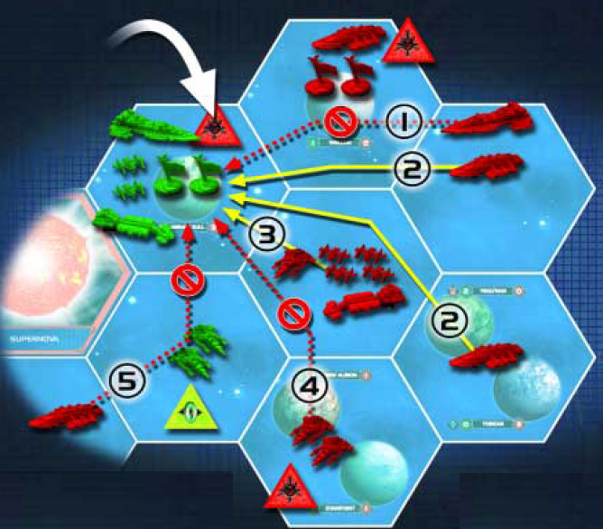
\includegraphics[width=0.87\textwidth]{activation_example.png}
\caption{ Example of Activation and Movement}
\label{fig:example_activation}
\end{figure}

\subsection{Status Phase} % (fold)
\label{sub:status_phase}

The Status Phase, when compared to either the Strategy or Action Phase, is a straightforward experience. It is during the Status Phase that many of the game functions are "reset," such as players refreshing Planet Cards, discarding Command Counters from the board, etc. It is also during the Status Phase that players may gain victory points by meeting the requirements of a Public and/or Secret Objective Card. To resolve the Status Phase, follow the Status Sequence below:
\subsubsection{The Status Sequence}
\begin{enumerate}
    \item  Qualify for Public/Secret Objective Cards
\item Repair Damaged Ships
\item Remove Command Counters
\item Refresh Planet Cards
\item Receive 1 Action Card and 2 Command Counters
\item Redistribute Command Areas
\item Return Strategy Cards
\end{enumerate}

\subsubsection{Qualify for public/secret Objectives} % (fold)
\label{sub:qualify_for_public_secret_objectives}        
In the order of play, each player may announce that he has met the requirements of one face-up Public Objective Card and/or his Secret Objective Card.
After a player announces that he has met the objectives of a face up Public Objective Card, he must prove to his opponents that his claim is valid.
After doing so, the player places one of his Control Markers on the claimed Objective Card (indicating that he has claimed that objective), and then advances his Control Marker on the Victory Point Track the appropriate number of spaces.
Once a player has received Victory Points for a specific Objective Card, he may not qualify for that Objective Card again.
In addition, if a player has met the requirements of his Secret Objective Card, he may now reveal the card, prove that its objectives are met, and then claim its victory points.

\emph{Important Exception: A player may never qualify for a Public or Secret Objective Card if he does not control all the planets in his Home System.}

\subsubsection{Winning the Game}
When a player advances his Control Marker to the 10th step of the Victory Point Track, he has gained the power needed to claim the Imperial Throne on Mecatol Rex. The Winnaran Custodians will step aside for their new emperor, who must lead the galaxy to a new age of prosperity and peace.

As players, one at a time, qualify for Objective Cards by following the order of play, one player will always reach 10 victory points first. That player is the winner of the game, even if other players would also have achieved 10 or more victory points later in the order of play.

It is also possible for a player to win the game during this step if he is the first to meet the requirements of either the “Supremacy” or “Domination” card (provided that either card is face up in the common play area).

\begin{FFGbox}
\subsubsection{The “Imperium Rex“ Objective Card}
While the Primary Ability of the Imperial Strategy card is resolved, it is possible that the “Imperium Rex” objective card is drawn from the Objective Deck. When this card is drawn, the game ends immediately and a winner is declared The winner is the player who has the most victory points (the active player does not receive the 2 victory points). If there is a tie, then the greater number of resolved Objective Cards breaks the tie; if there is still a tie, then the greater number of planets, then unused Command Counters, and then the total number of Command Counters on a player's Race Sheet. If still tied, then the game ends in a draw between the tying players.
\end{FFGbox}

\subsubsection{Repair Damaged Ships}
All damaged Dreadnought and War Sun units are returned to their normal upright position on the game board. They are no longer considered to be damaged.

\subsubsection{Remove Command Counters}
Each player now removes all his Command Counters from the game board, placing them in his reinforcements pile.


\subsubsection{Refresh Planet Cards}
Each player refreshes his exhausted Planet Cards by turning them face up.

\subsubsection{Players receive 1 Action Card and 2 Command Counters}
Each player now receives one Action Card from the Action Card deck and two Command Counters from his reinforcements (placing each Command Counter in either of the three appropriate areas of his Race Sheet).

\subsubsection{Redistribute Command Areas}
Each player (in order of play, if necessary) may now redistribute the Command Counters between the Strategy Allocation, Command Pool, and Fleet Supply areas on his Race Sheet. If a player reduces the number of Command Counters in his Fleet Supply, remember to check that all of his fleets on the board are in compliance with his new fleet size limit.

\subsubsection{Return Strategy Cards}
Each player now returns his Strategy Card to the common play area. Here the eight Strategy Cards will be ready for the beginning of the next game round.


\subsection{End of a Round}
After the Status Phase has been completed (and provided no winner has yet emerged), the game round is over and another game round begins with a new Strategy Phase. In this way, the game is played over a series of game rounds until a winner has been determined.


\chapterimage{board.jpg} % Chapter heading image
\chapter{Combat}


\section{Space Battles}
If the active system contains ships belonging to the active player and ships belonging to an opponent, a
Space Battle must be fought.

A Space Battle is fought over a consecutive number of combat rounds until only ships of one player remain (or the ships of both players have been simultaneously destroyed).

\subsection{Before Combat}
Before the actual Space Battle begins, resolve any pre-combat actions such as Destroyer Anti-Fighter
Barrage and then Sabotage Runs (the Sabotage Run is an optional rule found on page 63).
See also Chapter 15.2 Combat on Page 99 for detailed pre-combat actions order.

\subsubsection{Destroyer Anti-Fighter Barrage}

Both attacker and defender are allowed to use Destroyer Anti-Fighter Barrage, see Chapter 11.7 Destroyer Unit (Page 51).

Before the first round of Space Battle, roll two dice for each Destroyer unit in the battle. For every result equal to or higher than the Destroyer's combat value (all combat values can be found on the unit table on every player's Race Sheet), the opponent must take one Fighter unit as an immediate casualty. Such eliminated Fighter units are removed immediately and placed back among a player's reinforcements; they do not receive return fire and will not participate in the upcoming Space Battle.

A fleet containing no Fighter units is unaffected by pre-combat Destroyer fire.
\subsection{Battle Round}
After finishing any "before combat" actions, continue to the actual combat. A Space Battle always follows the Space Battle Sequence:
\subsubsection{The Space Battle Sequence}
\begin{enumerate}
    \item Announce withdrawals/retreats
    \item Roll combat dice
    \item Remove casualties
    \item Execute withdrawals/retreats
\end{enumerate}
After step 4, if both players still have ships remaining in the system, repeat the Space Battle Sequence until only one player has ships remaining, or all ships in the system have been destroyed.

Below, each step of the Space Battle Sequence is described in detail:


\subsection{Announce Retreats/Withdrawals}
The attacker first has the option to announce his withdrawal from battle. If the attacker chooses \emph{not} to declare a withdrawal, then the defender may declare a retreat. Note that if the attacker does decide to withdraw, the defender may not declare a retreat. Any actual withdrawals/retreats occur at the last step of the combat phase. This means that all Space Battles will have at least one round of combat.

\subsection{Roll Combat Dice}
During this step, both players simultaneously roll one combat die for every one of their spaceships in the battle (with the exception of the War Sun, which rolls three dice). For each result that is equal to or higher than the combat value of its ship, a "hit" is scored (all base combat values can be found on the unit table on a player’s Race Sheet). Players must remember the total number of successful hits as they move to the next step.

\emph{Example: The attacking player has a fleet of three Cruisers and one Dreadnought. During the first battle round, he rolls for his attacking ships. He takes three dice for the Cruisers (Combat Value 7) and rolls a 2, 5, and 7 -- one hit. Then he takes one die for his Dreadnought and rolls a 6 -- a hit. The attacking player announces that he has inflicted a total of two hits on the defending fleet. The defending player has two Fighters (supported by a Space Dock in the system) and one Destroyer. He takes two dice for the Fighter units and rolls a 3 and a 5 -- both misses. Then he takes one die for his Destroyer and rolls a 0 (a 10) a hit. The defending player announces that he has inflicted one total hit on the attacking fleet.}

\subsection{Remove Casualties}
Each player must now take a number of casualties equal to the number of hits scored by the opponent in step 2. First the attacking player removes his casualties. For every casualty, he must destroy one of his ships of his choice or damage one of his Dreadnoughts or War Suns (if a damaged Dreadnought or War Sun receives a second hit, it is destroyed). Destroyed ships are placed among a player's reinforcements, and become available for production once again. After the attacking player has removed all his casualties, the defending player must then remove his casualties.
Note that whenever a player removes casualties in TI, the casualty is always determined by the affected player. Since Fighters are the cheapest unit to produce, they make effective "cannon fodder" and are thus typically among the first units to be chosen as casualties.

\emph{Example: The defending player scored one hit. The attacking player then chooses to damage his Dreadnought (soaking up a casualty). The attacker scored a total of two hits. The defending player chooses to remove two Fighter units as casualties and places them back with his reinforcements.}

\subsection{Execute Withdrawals/Retreats}
If the attacking player announced a withdrawal or the defending player announced a retreat during step 1 of the Space Battle Sequence, that player may now execute the withdrawal/retreat, following the rules below.

\begin{itemize}
\item A withdrawal or retreat is not allowed if, at this point in the battle, the opposing player has no units left in the system. Even if a player announced a withdrawal or retreat at the beginning of the combat round, if he has somehow managed to destroy all the opposing units, the withdrawal/retreat is cancelled and the units must remain in the system.
\item When executing a withdrawal or retreat, a player must withdraw his entire fleet to an adjacent system that has previously been activated by the withdrawing/ retreating player that contains no enemy ships (but it can contain enemy planets with GFs, PDS and Space Docks). If a player has no previously activated systems adjacent to the contested system, he may not withdraw or retreat. (Changed in the Online-Errata: In former Versions there was no constraint, the system a player is withdrawing/retreating to, must not contain any enemy ships.)

    \item 
\end{itemize}
After a successful withdrawal or retreat, make sure that the withdrawing/retreating player is still in compliance with his Fleet Supply (see rules for Fleet Supply on page 35) and has sufficient Fighter capacity (see the Fighter unit description on page 50) in the new system. If not, he must immediately destroy the excess ships.

\section{End of Space Battle}
After the first Space Battle round is completed, if both players still have surviving ships in the system, another Space Battle round begins. This continues until only one player has ships in the system (or the ships of both players have been eliminated).

\begin{FFGbox}
\subsection{Receiving Planet Cards}
Whenever a player receives a Planet Card, by either successfully taking over a neutral planet or by successfully invading an enemy planet, he claims the corresponding Planet Card and places it exhausted in his play area. A newly claimed Planet Card is always received exhausted, even if the previous owner had not yet exhausted it.
\end{FFGbox}


\subsection{Space Battle Example}

\begin{figure}[h]
    \centering
    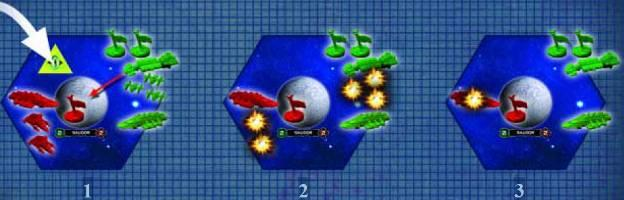
\includegraphics[width=0.77\textwidth]{battle_example.jpg}
    \caption{Space Battle Example}
    \label{fig:space_battle_example}
\end{figure}

\begin{enumerate}
    \item In this example, the Xxcha player has just activated a N’orr system, moving a fleet of one Carrier unit (carrying two Ground Forces), three Fighter units (also supported by the Carrier) and one Cruiser unit. As the N’orr has two Destroyer units in the battle, and the Xxcha has Fighter units, the N’orr Destroyers each will roll two dice for their pre-combat “Destroyer Anti-Fighter Barrage.” The results are 2, 2, 5, and 6 (all misses). The players then proceed to the first step of the Space Battle Sequence. The Xxcha player announces that he will not withdraw, and the N’orr player announces that he does not wish to retreat.

\item The Xxcha player now rolls combat dice for his units. His Fighters roll a 3, 5, and a 10 (one hit), his Carrier a 6 (a miss), and finally his Cruiser a 8 (one hit). The Xxcha player announces that he has made 2 successful hits. Then the N’orr player rolls three combat dice for his spaceships. The N’orr Cruiser rolls a 8 (a hit) and the two Destroyer units roll a 9 and a 10 (both hits). The N’orr player announces that he has made 3 successful hits. As casualties, the Xxcha player elects to destroy three Fighter units. The N’orr player removes his two Destroyer units.

\item The second round of Space Battle combat now begins. The Xxcha player declares that he will not withdraw and the N’orr that he will not retreat. The Xxcha player then proceeds to roll a 9 with his Cruiser (hit), and 1 with his Carrier (a miss). The N’orr player rolls a 3 with his Cruiser (a miss). As he must sustain one casualty, the N’orr player must destroy his remaining Cruiser, and the Space Battle is now over with the Xxcha player victorious. During the Planetary Landings step of the Activation Sequence, the Xxcha plans to land the two Ground Forces on the N’orr planet, starting an Invasion Combat.

\end{enumerate}



\section{Invasion Combat}
After the active player has landed one or more Ground Force units during the Planetary Landings step of a Tactical Action, an Invasion Combat must be fought if the destination planet holds any enemy Ground Force units. Invasion Combat is executed almost identically to Space Battle, with the notable exception that no withdrawals or retreats are allowed.

\subsection{Before Combat}
Before the actual Invasion Combat begins, players must resolve pre-combat actions such as planetary bombardments and defensive PDS fire.

\subsubsection{Bombardments}
Dreadnought and War Sun units in the activated system may bombard a planet before the player undertakes Invasion Combat (exception: a War Sun unit may bombard a planet even if no Invasion Combat is about to take place). Simply roll one combat die for every Dreadnought, three for every War Sun, and remove one enemy Ground Force on the contested planet for every result equal to or higher than the combat value of the bombarding unit. Remember that a Dreadnought may not bombard a planet that contains at least one enemy PDS due to the presence of a planetary shield. Ground Forces destroyed by bombardment are removed immediately, do not receive return fire, and will not participate in the upcoming Invasion Combat.

\subsubsection{PDS Fire}
After the attacking player has finished his bombardment, the defending player may fire a single shot with each PDS unit on the contested planet. The defending player rolls a die for every PDS unit present, and for every result equal to or greater than the combat value of the PDS unit, an invading Ground Force is destroyed. Attacking Ground Force units destroyed by defending PDS do not receive return fire and will not participate in the upcoming Invasion Combat.

\subsection{Invasion Combat Round}
After any bombardment and defensive PDS fire has been resolved, the players proceed to the Invasion
Combat. Like a Space Battle, Invasion Combat is fought over a series of consecutive combat rounds until only one player's Ground Forces (or none) remain. To resolve an Invasion Combat round, follow the Invasion Combat Sequence:
\subsubsection{Invasion Combat Sequence}
\begin{enumerate}[]
\item Roll combat dice
\item Casualties are removed
\end{enumerate}

\subsubsection{Roll Combat Dice}
Both players simultaneously roll one die for every friendly Ground Force unit on the planet. For every result equal to or higher than the combat value of the Ground Force unit, the player scores a "hit." Players must remember their total number of successful hits as they move to the next step.

\subsubsection{Remove Casualties}
Each player must now take a number of Ground Force unit casualties equal to the number of hits scored by the opponent in step 1. Casualties are, as always, returned to a player's reinforcement pile.
If, at this point, both players still have Ground Force units remaining on the planet, another Invasion Combat round is initiated. This continues until only one (or no) player has Ground Force units left on the planet.

\subsubsection{Invasion Success?}
If all defending Ground Forces were destroyed and at least one attacking Ground Force survived the battle, the invasion is a success. All defending PDS units and any Space Dock on the planet are immediately destroyed. The attacking player then claims the Planet Card from the previous owner and places it, exhausted, into his play area. Since combat is simultaneous, it is possible that all the Ground Forces on both sides were destroyed. If this is the case, the defending player retains control over the planet and simply places one of his Control Markers on the vacant planet to indicate this.


\chapterimage{rexbanner.jpg}
\chapter{Other Game Concepts and Rules}
\section{Races}


\begin{SEbox}
\subsection{Winnaran Yellow Technology Specialty}
The Winnaran home world is unique in that it is the only planet with a yellow (general) technology specialty. 
This yellow technology specialty works exactly like the red, green, and blue technology specialties except that the yellow technology specialty does not count for the purpose of fulfilling objectives.

\subsection{Saar Space Docks}
As described on their race sheet, the Clan of Saar’s Space Docks have a base movement of 1. The following rules also pertain to Saar Space Docks:
\begin{itemize}
	\item Saar Space Docks may only be built in a system containing a planet that you have controlled for the entire game round.
	\item Saar Space Docks do not count as ships and therefore do not count towards Fleet Supply and do not participate in Space Battles.
	\item Saar Space Docks are never blockaded; they are simply destroyed if present with enemy ships.
	\item Ground Forces and PDS units built in systems containing Saar Space Docks may be placed on any planet you control in the system, or they may go on a Carrier. 
	If you do not have a planet or Carrier in the system to place Ground Force or PDS units on, you may not build them.
\end{itemize}
\end{SEbox}
\begin{STbox}
	
\subsection{Arborec Green Technology Specialty}
The Arborec home world is unique in that it is the only home planet with a green Technology 
specialty.
This green Technology specialty works exactly like it would on any other planet and can even count for the purpose of fulfilling objectives.

\subsection{Ghosts of Creuss Home Systems}
The Ghosts of Creuss have two separate Home Systems connected by a “D” Wormhole.
Both of these systems are considered Home Systems for the purpose of card and game effects. During setup, the Ghosts of Creuss player only places the hexagonal tile in the galaxy.
He places the non-hexagonal tile in front of him.
Also, the “D” Wormhole is considered a Wormhole for the purposes of card and game effects.
\end{STbox}

\section{Systems}
There are three types of systems in TI3:

\subsection{Home Systems (Interior Yellow Border)}
These represent the starting systems for each of the 10 great races.
At the beginning of the game, players randomly draw one of these systems to determine which race they will play.

\subsection{Special Systems (Interior Red Border)} \index{special sysytems}
The Special Systems represent five unique types of interstellar terrain, governed by the following rules:

\subsubsection{Asteroid Field} \index{asteroid field}
A player's ships may not move through an Asteroid Field unless that player has gained the Antimass Deflector technology. 
If a player does have the required technology, he may move his ships through an Asteroid Field, but it is never possible, by any means, for a ship to end its movement in an Asteroid Field. An Asteroid Field may never be activated.

\subsubsection{Supernova} \index{supernova}
These fiery dying stars are incredibly dangerous and absolutely impassable. A Supernova may never be activated.

\subsubsection{Nebula} \index{nebula}
A Nebula is governed by the following rules:
\begin{itemize}
	\item A Fleet defending a Nebula receives +1 to its combat rolls during any Space Battle here
	\item Ships can never move through a Nebula (but ships can move into a Nebula via normal activation)
	\item A ship leaving a Nebula always has its movement reduced to 1 (regardless of technology modifiers and Action Cards).
\end{itemize}

\begin{SEbox}
\subsubsection{Ion Storm} \index{ion storm}
An Ion Storms is governed by the following rules:
\begin{itemize}
	\item Ships may never move through an Ion Storm (however, ships can move into an Ion Storm via normal activation).
	\item PDS Cannons may never be fired at ships inside an Ion Storm.
	\item Fighters do not roll any dice during combat inside an Ion Storm. 
	However, Fighters may still be taken as casualties.
\end{itemize}
\end{SEbox}
\begin{STbox}
\subsubsection{Gravity Rift} \index{gravity rift}
A Gravity Rift is governed by the following rules:
\begin{itemize}
    \item Ships may move into and through a Gravity Rift.
	\item When a ship moves out of (or through) a Gravity Rift, its controlling player must roll a die. 
	On a roll of 1–5, the ship is destroyed. 
	If there are multiple ships moving out of a Gravity Rift on the same activation, a separate roll must be made for each ship. 
	If a Carrier is destroyed, all Ground Force and Fighter units being carried by that Carrier are also destroyed.
\end{itemize}
\end{STbox}

\subsection{Regular Systems}
Regular systems are either empty, or contain one to two planets (see the "Planets of Twilight Imperium" sidebar for more information).
Some regular systems also contain an end of either the Alpha or Beta Wormhole.
The large majority of the TI galaxy consists of regular systems, and they form the battlegrounds and points of contention for the great races.
Although considered a regular system, the Mecatol Rex system always forms the centre of the galaxy and is never randomly distributed to players before the galaxy is created.

\begin{SEbox}
	
\subsection{Refresh Abilities} \index{refresh abilities}
Some regular systems have Refresh abilities that may be used during the Status Phase.
A Refresh ability is indicated on the hex by an icon to the right of the planet name and is detailed in the text of the corresponding planet card.
During the Status Phase, immediately after refreshing planet cards, you may exhaust one or more planets with the Refresh ability to gain the special abilities listed on their planet cards.
When you exhaust a planet to gain its ability, you do not gain its re sources.
Refresh abilities may provide 2 Trade Goods, 2 Shock Troops, 2 Ground Forces, or 2 Fighters.
If the Refresh ability provides units, the units must be placed on the planet that was exhausted to produce them.
If you are not playing with the Shock Troops option (see page 65), then Refresh abilities that provide Shock Troops provide Ground Forces instead.

\subsection{Trade Stations} \index{trade stations}
Two regular systems contain Trade Stations (Tsion and Sumerian). Trade Stations have a white name box and a space for a Control Marker. Trade stations follow the rules below:
\begin{itemize}
	\item No Distant Suns Domain tokens are placed on Trade Stations.
	\item Trade Stations have a special Refresh ability that gives the controller 2 Trade Goods if exhausted during the Status Phase. See Refresh abilities (above).
	
	\item Trade Stations may never be invaded.
	Instead, whenever a player has ships in a system in which no other player’s ships are present, he immediately places his Control Marker on the station (and gains the corresponding planet card in its exhausted state).
	The Control Marker stays on the station until another player becomes the only player with ships in the system (at which point the other player places his Control Marker on the system and gains the corresponding planet card in its exhausted state).
	Control Markers may also be removed from Trade Stations by certain abilities and cards.
	
	\item Capturing a Trade Station from an opponent does not break a trade agreement with that opponent.
	\item Ground Forces, Space Docks, and PDSs may not be placed on Trade Stations.
	\item Aside from the above exceptions, Trade Stations are still considered planets (with planet cards) for the sake of abilities and other cards that target planets.
	For example, a player can target a Trade Station with Peaceful Annexation (a power on the new Diplomacy Strategy Card in this expansion) or the Local Unrest Action Card. 
	(Note, however, that using an ability such as Peaceful Annexation – which gives you control of a planet – on a Trade Station in which another player is the only player with ships in the system is pointless, since that player will immediately regain control of the station.)
\end{itemize}


\end{SEbox}

\section{Planets}

\begin{figure}[h]
    \centering
    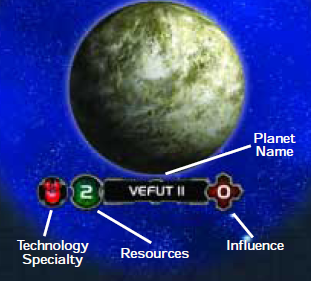
\includegraphics[]{planet.png}\\
    \caption{Planets}
    \label{fig:planets}
\end{figure}



% The real points of interest in the TI galaxy are its planets. 
% Each planet is printed with its name, resource value (R), influence value (I), and possibly a technology specialty (to the left from resource value).
% When a player successfully invades a planet (neutral or enemy), he immediately claims its corresponding Planet Card.
% Resources represent a planet's economic surplus, which can be used by its owner to purchase units and technology. 
% Influence represents a planet's population, knowledge base, and/or political importance. Influence is used to acquire Command Counters, to play certain Action Cards, and to provide vital votes at the Galactic Council.
% Technology specialties represent a certain local knowledge or a natural resource important to a specific area of science.
% This provides the owner of the planet with a discount resource towards purchasing advances of that technology type.


% \section{Wormholes}
% In TI, Wormholes are spatial anomalies that connect distant areas of space.
% A system containing one end of a Wormhole is considered adjacent (even for the purposes of a transfer action) to a system containing another end of its Wormhole type (Alpha or Beta).
% For example, a ship with a movement rate of 1 may move from a system containing a Beta Wormhole, directly to another system containing a Beta Wormhole (remember that all movement is still part of an Activation Sequence in which ships must end their movement in the activated system).
% If only one Wormhole of a type is in play, it has no function and is ignored.

% \section{Unit Limitations}
% Except for Fighters and Ground Forces, players are limited to the number of units provided in the game. If all of a player’s units of a specific type are on the board, that player may not produce additional units of that kind until one is destroyed and returned to the player's reinforcement pile.

% \subsubsection{Scuttling units} \index{scuttling units}
% At any time during the Status Phase, players are allowed to scuttle (destroy) any of their own units on the board.
% Scuttled units are simply returned to the player’s reinforcement pile and become available for production during the next Action Phase.
% Players may not scuttle units until step 1 of the Status Sequence (Qualify for Public/Secret Objectives) is complete.

% \section{Fighter and Ground Force Supplement Counters}
% Unlike every other unit type, players are allowed to build more Fighter and Ground Force units than supplied with the game.
% To build these additional units, players must use the Fighter or Ground Force Supplement Counters.
% These counters are neutral, can be used by any player, and are governed by the following rules: 
% \begin{itemize}
% 	\item The presence of a Supplement Counter simply states "there is one additional unit of this type here!" 
% 	\item There must always be at least one actual unit (controlled by the same player) of the appropriate type in the same system, or on the same planet, as a Supplement Counter. 
% 	\item Players may, at any time, replace any number of Ground Forces and/or Fighters in a system/planet with an equal number of Fighter/Ground Force Supplement Counters as long as at least one original unit remains. 
% 	\item The actual units are placed back among a player's reinforcements, and the appropriate Supplement Counters are taken from the common play area and placed on the board in the same spot. 
% 	\item Likewise, players may, at any time, replace Supplement Counters on the board with actual units from their reinforcements (if able). Players must do this when they want to split the forces without sufficient actual units present.
% \end{itemize}

% Be careful that, in multi-planet systems, each planet with Ground Force Supplement Counters contains at least one actual Ground Force unit.

% It is only really necessary for a player to use Supplement Counters if he is about to run out of actual units in his reinforcement pile.
% In some instances, it is possible that there is too little physical room on a given planet/system, and that a player may wish to create more room by replacing some Ground Force/Fighter units with counters.
% A player may, during production, produce Supplement Counters, but only if the producing system/planet contains at least one actual unit of that type after the production is complete.
% As stated, Supplement Counters are simply additional units of the indicated type, and therefore also must behave under all the same rules as the actual unit.
% In other words, Fighter Supplement Counters must have sufficient Carrier/Space Dock/War Sun capacity in order to exist.
% Ground Force Supplement Counters must be transported by a Carrier in order to move to another planet, etc.
% Note that when Supplement Counters are transported by a Carrier or War Sun, at least one actual unit of that type must also be transported by that same Carrier/War Sun.
% If a Supplement Counter is on system/planet without an actual unit of its type, it is immediately removed.
% An easy way to manage your Supplement Counters is to always place them under an actual unit of their type in the area.
% As long as a Supplement Counter is under an actual unit of its type, it will always conform to the rules.

% \section{Command Counters}


% At the start of the game, players are each provided with a total of 16 Command Counters. 
% During the game, these counters will be either on a player's Race Sheet or with his reinforcements.

% Whenever a player receives a Command Counter from his reinforcements, he must immediately place it on his Race Sheet in one of the three following areas:
% \begin{itemize}
% 	\item The Strategy Allocation Area
% 	\item The Fleet Supply Area
% 	\item The Command Pool Area
% \end{itemize}

% These three areas represent three distinctly different vital areas of managing your race.
% Once a player places a Command Counter in one of these areas, he may not move it to a different area until the upcoming Status Phase.
% Decisions on where to place and how to spend Command Counters are among the most important that a player will make during the game.
% When a player spends a Command Counter, or uses a Command Counter to activate a system, he must remove the counter from the appropriate area of his Race Sheet and return it to his reinforcements. In detail, the effects and rules for each of the three areas are as follows:

% \subsection{Fleet Supply Area} \index{fleet supply area}

% The number of Command Counters in a player's Fleet Supply area dictates the maximum number of ships (not including Fighters) that a player may have in any given system on the board.
% A player may never move units, build units, or otherwise acquire units in any system so that the number of ships herein (again, excluding Fighters) exceed the number of Command Counters in his Fleet Supply area.
% If, for any reason, the number of ships in a system should exceed the number of Command Counters in a player's Fleet Supply, the owner of those ships must immediately remove enough ships from the system (by placing them back with his reinforcements) until the number of ships is again in compliance with the number of Command Counters in his Fleet Supply area.
% When a player places a Command Counter in his Fleet Supply area, it is placed with the "Fleet" side up, to indicate that it is a part ofthe Fleet Supply area.
% In this way, other players can easily identify your fleet limit from across the table, and it helps prevent your counters from mixing with the Command Counters in the two other areas.
% As a player increases the number of Command Counters in his Fleet Supply area, he may increase the size of his fleets on the board correspondingly.
% It is important to note that a player may have any number of active fleets on the board, as long as each fleet contains a number of ships that is equal to, or less, than its owner's Fleet Supply limit.
% As noted, Fighter units do not count toward the Fleet Supply limit. 
% A player may thus have any number of Fighter units in a given system, as long as he has the capacity to support them (see \namepageref{sec:fighter_unit}).

% \subsection{Command Pool Area} \index{command pool area}
% After a player decides to take a Tactical or Transfer Action during the Action Phase, he must take an available Command Counter from his Command Pool in order to activate a system on the board.
% If a player has no Command Counters remaining in his Command Pool, he is not able to take Tactical or Transfer Actions.
% In other words, the number of Command Counters in a player's Command Pool dictates the amount of activity he can initiate on the board.

% \subsection{Strategy Allocation Area} \index{strategy allocation area}
% Generally, Command Counters in the Strategy Allocation area are spent to execute the Secondary
% Abilities of Strategy Cards.
% Some races have special abilities and some Action Cards require their players to spend Command Counters from their Strategy Allocation area for other effects.

% \section{Spending Resources and Influence}
% Throughout a game of TI, you will need to spend resources and influence for many different purposes. 
% Both resources and influence are provided by the planets under your control, and you will use their corresponding Planet Cards to keep track of your expenditures.

% \subsection{Exhausting Planets} \index{exhausting planets}
% Whenever you want to spend influence or resources you must exhaust one of your Planet Cards by turning it face down.
% This provides you with the resources or influence of that planet. 
% Each Planet Card (and the planets on the board themselves) shows the specific information on how many resources and how much influence is gained from exhausting that specific planet (see the diagram above). 
% A face down Planet Card cannot be exhausted again until it is refreshed during the Status 
% Phase (or by another effect). When a card is refreshed, it is simply returned to its face-up position. 
% When you exhaust a planet for its resources or influence, it provides you with all of its resources or influence. 
% You cannot use the resources or influence of a planet partially, nor can you save a portion for later.
% Note that when exhausting a planet, it will provide you with either its resource value or its influence value, but not both. 
% Before exhausting a planet, you must announce whether you are exhausting it for its resources or for its influence (in most cases it is clear for what purpose you are exhausting a planet).

% \subsection{Paying Costs} \index{paying costs}
% Whenever a player wishes to spend resources or influence, he simply announces the total amount of resources/influence that he wishes to spend, and then exhausts the number of Planet Cards with that (or greater) combined amount of resources/influence. 
% In other words, when a player is producing units at a Space Dock during the Production step of the Activation Sequence, he may simply announce how many resources he is going to spend in total. 
% Then he exhausts the appropriate number of planets and places the produced units on the board (see \nameref{sec:building_units} on page \pageref{sec:building_units}).
% This means that you are not producing (and spending resources on) a single unit at a time, but rather purchasing the production with one lump sum. 
% The same goes for spending influence. 
% Any spare resources or influence provided by an exhausted Planet Card are lost.

% \subsubsection{Special Note}
% You do not have to exhaust a specific Planet Card to pay for the cost of production at that exact planet; any resources will do.

% \todo{omitted an example for now}
% \todo{example image}

% \section{Action Cards}
% Throughout the game, players will come into possession of Action Cards.
% Action Cards should be kept hidden from other players. An Action Card can only be used given the specific circumstances (or phase) printed on each individual card.
% \emph{A player may never have more than 7 Action Cards at any one time.}
% If, after receiving additional cards, a player has more than 7 Action Cards in his hand, he must immediately choose and discard cards until he has 7.
% If a player at 7 cards is about to draw additional cards, he should draw and discard one Action Card at a time.
% A player may never play two identical Action Cards for the same situation and/or on the same entity during one round.

% \subsubsection{Example}
% A player cannot play two "Flank Speed" Action Cards on the same fleet in one Game round. The player may, however, play a “Flank Speed” on two different fleets in the same round.

% \subsubsection{Trade Good icon}
% Some Action Cards have a Trade Good icon printed on them. If not playing with the optional rule printed on the card, the card may be discarded instead of spending 1 Trade Good.

% \subsection{How to Play an Action Card}
% If a player wishes to play an Action Card, he must publicly announce that he wishes to play an Action Card.
% Then other players, at that time, may announce that they also wish to play an Action Card.
% After all players have been given the opportunity to announce that they are playing Action Cards, all the Action Cards are revealed and resolved in order of play.
% If Action Cards are about to played at a time where players do not have Strategy Cards, then resolve them in clockwise order starting with the Speaker.

% \subsection{Sabotage Action Card}\index{sabotage action card}
% A player \emph{does not have to announce} the playing of a Sabotage card.
% The Sabotage card is simply played immediately after an Action Card has been revealed, cancelling its effect.
% Then both cards are discarded.

% \subsection{"Play as an Action"} \index{play as an Action}
% Some Action Cards read “Play: As an action.” 
% This Action Card must played by its owner during the Action Phase instead of taking a regular action.

% \section{Political Cards an the Galactic Council}
% When the player who controls the Political Strategy Card executes his Strategic Action, a Political Card must be drawn and the Galactic Council convenes to debate and vote upon its agenda.

% \subsection{Political Agenda} \index{political agenda} \index{agenda}
% Every Political Card contains an agenda that requires a vote in the Galactic Council (i.e., the players).
% As the first step of convening the Galactic Council, the active player reads aloud the drawn Political Card and makes it clear what kind of vote is about to be cast. T
% here are two types of agenda votes:

% \subsection{"Elect" Votes} \index{elect votes}
% When a political agenda asks the Galactic Council to elect something or someone, each player may choose who or what to nominate (i.e., elect) when casting his vote.
% That player's entire vote is now attributed towards that subject.
% The subject with the highest number (not necessarily the majority) of the total votes is considered elected.
% After this, follow the instructions on the Political Card.

% \subsection{"For or Against" Votes} \index{for or against votes}
% Most agendas will ask the Galactic Council to vote for or against a certain agenda.
% In this type of vote, players indicate either “for” or “against” when casting their vote.
% The majority of all votes cast will decide the outcome.

% \subsection{Laws} \index{laws}
% Some agendas are "Laws."
% Laws represent permanent changes to the rules and/or flow of the game.
% When a Law is voted "for," first enact any effects of the "for" result and then place the Political Card face up in the common play area.
% The effects of this card are now permanent.
% If voted "against," resolve any effects that an "against" result may have and then discard the card.

% Although the council might have adopted a Law earlier in the game, the balance of power can later have shifted, and old Laws soon become unpopular.
% If this happens, how can the council reverse the old Law?
% Among the Political Cards, there are certain agendas that allow older Laws to be either re-evaluated or discarded.
% Note that these cards are few and that most enacted Laws are in the game to stay, so be careful how you vote.

% \subsection{Voting in the Galactic Council} \index{voting}
% After the active player has read the agenda out loud, the Galactic Council must resolve the agenda in the following way:

% Players first debate, threaten, lure, or convince each other to vote in their favour.
% Trade Good Counters may be used as "bribes" but no promises or agreements in TI are binding (even after receiving a bribe or payoff).

% Players then vote upon the agenda.
% Voting is done clockwise one player at a time, starting with the player to the left of the Speaker (thus the Speaker will always cast the last vote).
% When voting, a player has as many votes as the total combined influence value of all his unexhausted planets (and a minimum of 1 vote).

% \begin{itemize}
% 	\item When voting, a player must cast all his votes or none.
% 	\item Votes cannot be split.
% 	\item Voting does not cause your Planet Cards to exhaust.
% 	\item Trade Good counters cannot be used to gain additional votes.	
% \end{itemize}

% The Galactic Council is meant to be a fun, active engagement in which players forge alliances, use their political prowess, engage in sabrerattling, and "act their race."
% As powerful agendas are presented to the council, weaker players can seek to hurt strong neighbours politically via the enactment of damaging Laws or other agendas.

% \subsection{Abstaining and Tie Votes} \index{abstaining} \index{tie votes}
% A player may always choose to abstain from voting during any agenda.
% If so, his votes are simply not counted for purposes of resolving the agenda (including determining a majority).
% If there is a tie vote, even a tie of "0" (in which all players have abstained), the player holding the Speaker Token breaks the tie.

% \subsubsection{Rules and Cards}
% If the effect of a card seems to contradict the rules of the game, the card text is always correct.

% \section{Technology Advances} \index{technology advances}
% Before the game begins, each player is provided with an identical deck of 24 Technology advances, and each player starts the game with a few “Starting Technology” advances. 
% When a player has successfully acquired (or received at the start of the game) a Technology advance, he takes the respective Technology Card and places it face-up before him in his play area. 
% In this way, players will slowly accumulate Technology Cards, each providing a helpful advantage described on the card itself.

% Technology Cards are normally acquired during the resolution of the Technology Strategy Card, but can also be acquired via certain Action and Political Cards.
% \emph{Players may not give each other Technology advances.}

% There are four different technology areas, each attributed the following colour:

% \begin{description}
% 	\item[Red] Warfare Technology
% 	\item[Green] Biotechnology
% 	\item[Blue] Propulsion Technology
% 	\item[Yellow] General Technology
% \end{description}

% \subsection{Acquiring a Technology Advance}
% In general Technology advances are acquired when the Technology Strategy Card is executed during the Action Phase.
% The active player receives a free Technology advance, and other players may pay 8 resources to acquire one Technology advance.
% Most Technology advances (but not all) have prerequisite technologies. 
% Before a Technology advance can be acquired, a player must already have obtained all prerequisite technologies printed on the card.

% A player is not allowed to acquire a technology (via Action Cards, or otherwise) if he does not already have the prerequisite technologies face up in his play area.

% \subsection{Planetary Technology Specialities} 
% \index{planetary technology specialities}
% \index{technology specialities}

% Some planets have a technology specialty (a printed technology symbol by the planet itself and on the Planet Card).
% Technology specialties represent a certain local knowledge or a natural resource important to a specific area of science.
% The presence of a technology specialty gives the owner of the planet the ability to purchase a Technology Card (of the specific type: red, green, or blue) for 1 less than its normal cost when executing the secondary ability of the Technology Strategy Card.
% If a player controls multiple planets with technology specialties of the same colour/type, the cost to acquire that technology type is lowered by 1 for each such planet.

% Technology specialty discounts do not apply if the contributing Planet Card(s) is exhausted. 
% (It is not necessary to exhaust a planet with the technology specialty in order to receive the discount, nor is it necessary to exhaust that specific planet to buy the Technology advance).

% \subsection{The Yellow Technology Specialty} 
% \index{yellow technology specialty}
% The yellow (general) Technology specialty works exactly like the red, green, and blue Technology specialties except that the yellow Technology specialty does not count for the purpose of fulfilling objectives.

% \section{Trade Goods}\label{sec:trade_goods}
% \index{trade goods} 

% \subsection{Trade Goods Counters}
% Players may spend Trade Good counters from their Trade Goods area \emph{as a substitute for spending either one resource or one influence}.
% In this way, a player can pay for a Dreadnought unit by spending 5 Trade Goods from his Trade Goods area, or by exhausting Planet Cards for 3 resources, and paying the remaining 2 resources with Trade Goods (or any combination thereof).
% When a player spends a Trade Good, he simply moves it from his Trade Goods area to the common play area.
% Players are allowed to give other players Trade Goods from their Race Sheet at any time.
% This makes the Trade Goods counter a flexible currency with which to bribe, pay, or assist other players economically.

% \subsection{Receiving Trade Goods} \index{receiving trade goods}
% A player receives Trade Goods by simply taking required number of Trade Goods from the common play area and placing them on the Trade Goods area of his Race Sheet.

% \subsection{Running out of Trade Goods}
% There are exactly 88 Trade Goods in the game (40 + 12 in SE + 36 in SotT) if the Trade supply in the common play area is empty, then \emph{players cannot receive additional Trade Goods} until a player spends some and returns them to the common play area once more. 
% Since there is a limit to the total number of Trade Goods, it is important to adhere to the player order of executing the secondary ability of the Trade Strategy Card, which is always done in clockwise order from the active player.
% \todo{recheck TG count}

% \section{Trade Contracts and Trade Agreements}
% In TI, trading is an important avenue for players to gain additional resources and influence. 
% Trade can be used as important political leverage against hostile players or to help seal an important alliance.
% At the beginning of the game, each race is provided with two Trade Cards, each with a numerical trade value printed on the "trade agreement" side of the card (you may notice that some races have Trade Cards of differing trade values).
% At the beginning of the game, players should place these cards with the “Trade Contract“ side up in their playing area. 
% This side has no trade value, as players derive no value from their own Trade Cards.

% \subsubsection{Note}
% Information below about Trade Strategy Card only applies to strategy card from the Base game.
% Further reading: \namepageref{sec:trade_strategy}.

% \subsection{Opening Trade Agreements} \index{opening trade agreements}
% When the primary ability of the Trade Strategy Card is being resolved during the Action Phase, the active player may allow players (himself included) to forge trade agreements.
% A trade agreement is initiated between two players who agree to trade with each other.
% After agreeing to trade, each of the two players must give the partner one of their own Trade Cards.
% Upon receiving another player’s Trade Card, a player should place it before him with the trade agreement side face up.
% Only one Trade Card for each player may be exchanged, not more.
% Since every race has only two Trade Cards, each player may only have two active trade agreements at any one time.
% Before a trade agreement can be completed, the agreement must first be approved by the active player. 
% If approved (and that may take some bribes to the active player), the players may exchange Trade cards.

% \emph{Two players may only make one trade agreement with each other.}
% Thus, for a player to utilize both of his Trade Cards, he must make trade agreements with two different opponents. 
% If able, a player may initiate both of his trade agreements during the same execution of a Trade Strategy Card.
% It is important to note that since each player only has two Trade Cards, he cannot make more than two trade agreements.

% While executing the primary ability of the Trade Strategy Card, the first player receives Trade Goods for his trade agreements (the total trade value of any trade agreements in his play area) and 3 extra trade goods. 
% After the active player has completed the primary ability, the other players, clockwise from the active player, may execute the secondary ability of the Trade Strategy Card to receive Trade Goods for their trade agreements.

% Note that players are not allowed to collect trade income from trade agreements formed during the same action. It is not possible for a player to make a trade agreement during the primary ability of the Trade Strategy Card, and then immediately collect trade income from the new trade agreement by executing the secondary ability.

% \subsection{Breaking Trade Agreements}
% Any player involved in a trade agreement may unilaterally break the agreement during the Status Phase.
% Such a player simply announces that he is ending the agreement and immediately returns the Trade Card to its owner and retrieves his own Trade Card from the former trading partner (a player’s own Trade Cards are always returned with the “Trade Contract” side face up, as they provide no trade value for their owner).
% It is not possible for a player to automatically break a trade agreement with the Hacan race, as per the Hacan's special ability.

% If two trading players become involved in open war against each other (by one player initiating either a Space Battle or Invasion Combat against the other), a trade agreement between the two players is automatically broken (and the Trade Cards returned to their owners).
% The two players may later open another trade agreement, but this will again be broken if another Space Battle or Invasion Combat occurs between them. 
% Trade agreements with the Hacan player are broken in the event of open war between the Hacan and its trading partner.

% Note that only Space Battles and Invasion Combat will automatically break a trade agreement between two players.
% Playing Action Cards or taking shots with a PDS, etc., does not cause an automatic break.
% \emph{Invading a planet that contains only an enemy Control Marker is still considered Invasion Combat for purposes of cancelling trade agreements}.

% \subsection{Power of the Merchants Guild}
% When executing the primary ability of the Trade Strategy, the active player may choose to exercise his control of the Merchant’s guild in a destructive way, rather than facilitating the wealth of other races.
% As described in option “b” of the Trade Strategy Card, the active player, instead of receiving Trade Goods and opening trade negotiations, may instead choose to cancel every trade agreement in play.
% If the active player chooses this option, all Trade Cards (including those of the active player and the Hacan) are returned to their owners.

% \subsubsection{Definition of an “Empty“ System} \index{empty system}
% The TI rules and cards will sometimes refer to an “empty” system.
% An empty system is a system completely free of units, including units belonging to the active player.
% In other words, an empty system is one that is free from ship, Ground Force, PDS, or Space Dock units.
% The system may, however, contain planets, Control Markers, and Command Counters. 
% Special Systems are not considered empty systems.

% \section{Objective Cards}
% The Objective Cards represent the primary way for players to receive victory points.
% Each Objective Card (both Secret and Public) contains a requirement and a victory point award for meeting that requirement.
% The Public Objective Cards are slowly revealed as the Imperial Strategy Card is resolved during the Action Phase.
% During the first step of the Status Phase, players may qualify for the requirements of one revealed Public Objective Card in order to receive the corresponding victory points.
% Note that a player cannot gain victory points from a Public Objective Card that is not yet revealed.

% Some Objective Cards state “Now I…”.
% This requires a player to actually fulfil the requirement during the first step of the Status Phase.
% For example, one Objective Card reads “I now spend 20 Resources (2 victory points).”
% In order for a player to receive these two victory points, he must have enough Trade Goods and unexhausted planets to spend 20 resources during the first step of the Status Phase.
% A player may only receive victory points from a specific revealed Objective Card once per game.
% After collecting victory points from an Objective Card, a player should, to serve as a reminder, place one of his Control Markers on the card.

% \section{Secret Objective Cards}
% At the beginning of the game, each player receives a Secret Objective Card.
% A player is not allowed to show other players his Secret Objective Card until he is able to meet its objectives during the first step of the Status Phase.
% A player who reveals his Secret Objective Card without being able to meet its requirements loses his Secret Objective Card, which is placed back in the box. 
% Such a player will not be able to receive victory points from a Secret Objective for the duration of the game.
% During the Status Phase, a player may qualify for one Public Objective Card and/or his Secret Objective Card.
% A player cannot qualify for more than one Public Objective Cards in one round.

% \section{Race Sheet}
% The Race Sheet provides a wealth of useful information and is used to manage a player’s active Command Counters.
% Here is a brief explanation of the player Race Sheet:
% \begin{enumerate}
% 	\item \textbf{Race Title and Symbol.}
% 	The symbol and title of the represented race.
	
% 	\item \textbf{Starting Units and Special Abilities.}
% 	The starting units/technologies, and the special abilities of the race.
	
% 	\item \textbf{Phase and Sequence Tables.}
% 	A detailed overview of the important phases and sequences of the game round.
	
% 	\item \textbf{Unit Data.}
% 	A detailed chart with the costs, combat value, movement rating, and special abilities of each unit type.
	
% 	\item \textbf{The Strategy Allocation Area.}
% 	Command Counters herein can be spent to execute the secondary abilities of Strategy cards (and a few other special functions).
	
% 	\item \textbf{The Fleet Supply.}
% 	Command Counters herein are flipped to their “Fleet” side, so that they do not mix with the other Command Counters on the Race Sheet.
% 	The number of Command Counters herein determines the allowable size of a player’s fleets.
	
% 	\item \textbf{The Command Pool.}
% 	A player must spend Command Counters from this area when activating systems on the game board (when taking a Tactical or Transfer Action).
	
% 	\item \textbf{The Trade Goods Area.}
% 	When a player receives a Trade Good counter, it is placed in this area.
% 	A player may give Trade Goods to other players at any time, or use Trade Good as a substitute for spending either one resource or one influence.
% \end{enumerate}

% \begin{figure}[h]
% 	\includegraphics[width=\textwidth]{race_sheet}
% \end{figure}




% \chapter{Rules for Units}
% Following is a detailed breakdown of the characteristics and rules for the 9 different unit types in TI that players have at their disposal.

% \section{Space Dock}
% \begin{wrapfigure}{L}{0.3\textwidth}
% 	\vspace*{-10pt}
% 	\includegraphics[scale=0.8]{/units/dock}
% 	\vspace*{-10pt}
% \end{wrapfigure}

% \unitdesc{3}{4}

% The Space Dock unit represents a military industrial complex, shipyard, and recruiting station in close orbit of a specific planet. 
% In order to build units (other than another Space Dock) in a given system or on a specific planet, a Space Dock must be present there.

% \subsection{Building a new Space Dock}
% In order to build a new Space Dock on a planet, the following requirements must be met:
% \begin{enumerate}
% 	\item The system (that contains the planet on which you want to build the Space Dock) has just been activated, and is currently at the “Production” step of the Activation or Transfer Sequence.
% 	\item The active player must have controlled the planet for the entire current round. Thus, it is not possible to build a Space Dock on a planet that has just been acquired during the current round.
% 	\item The planet does not already contain a Space Dock (only one Space Dock per planet is allowed).
% 	\item The system does not contain any enemy ships.
% \end{enumerate}

% If these requirements are met, the activating player may take an available Space Dock from his reinforcements, spend 4 resources, and place the Space Dock on the chosen planet. 
% Next round the Space Dock may begin producing units for its owner. 
% It is important to remember that a Space Dock is tied to a specific planet and is not considered to be “in space” and so does not participate in Space Battle, nor can it be attacked directly by enemy ships.

% \subsection{Building Units at a Space Dock} \label{sec:building_units}
% In order to produce new units (other than a new Space Dock), players must activate (via a Tactical or Transfer Action) a system that contains at least one friendly Space Dock. 
% As the last step in resolving the activation of the system, the activating player may spend resources to build units at the Space Dock, governed by the following rules:
% \begin{itemize}
% 	\item A Space Dock may only build a number of units (regardless of type) equal to the resource value of its planet plus two. 
% 	This means that a Space Dock located on a planet with a resource value of 3 may produce up to 5 different units (3 for the resource value of the planet, plus 2 for the Space Dock itself). 
% 	This restriction is for the number of units, regardless of their total resource cost. 
% 	Thus the above planet with a production limit of 5 may produce 5 Dreadnoughts or 5 Fighters (or any combination of those, and other, units).
	
% 	\item New spaceships (Fighters, Cruisers, Carriers, Destroyers, Dreadnoughts, and War Suns), when built, are placed directly (and always exist) in space. 
% 	Each system represents one area of space. Unlike Ground Forces, PDS, and the Space Dock itself, spaceships are never considered to be on, attached to, or affiliated with a planet in their current system.
	
% 	\item Ground Force and PDS units are always built and placed on the planet containing the Space Dock.
	
% 	\item Note that when purchasing either Fighter or Ground Force units, 1 resource provides two units. 
% 	If, due to the production limit of a Space Dock, a player wishes to only purchase 1 Ground Force or Fighter unit, the single unit still costs 1 resource. 
% 	A player may not “mix and match“ when purchasing Ground Forces and Fighters, such as purchasing one of each for only one resource.
% \end{itemize}

% \subsubsection{Note}
% Ground Force and PDS units cannot move to another planet (including other planets in the same system) unless transported by a Carrier or War Sun.

% Other Rules for Space Docks:
% \begin{itemize}
% 	\item 
% 	A Space Dock has the capacity to support 3 Fighter units in its system (see later).
	
% 	\item 
% 	If a system contains at least one enemy spaceship, all friendly Space Docks in that system are considered under blockade, and may not produce spaceship units while the enemy units are in the system. 
% 	A Space Dock under blockade may still build Ground Forces and PDS on its planet during the Production step of the Activation Sequence.
% \end{itemize}

% \subsubsection{Strategy Tip}
% Cruisers and Destroyers are especially useful for swooping in from afar to blockade your Space Docks. 
% Be cautious if fast enemy ships are within range, and try not to rely on just one Space Dock for your production, especially later in the game.

% \section{Ground Forces}
% \begin{wrapfigure}{L}{0.3\textwidth}
% 	\vspace*{-10pt}
% 	\includegraphics[scale=0.8]{/units/ground_force}
% 	\vspace*{-10pt}
% \end{wrapfigure}

% \unitdesc{12 (plus supplement counters)}{1 (produces two Ground Force units)}

% The Ground Force unit represents a player's military and occupational forces. 
% It is an essential unit necessary to take over neutral planets, invade enemy planets, or defend your own planets against enemy invasion. 
% Ground Forces are governed by the following rules:

% Ground Forces, when produced, are placed on the planet of the producing Space Dock. 
% Ground Forces are primarily transported around the galaxy by Carrier units (although the War Sun unit, as well as certain Technology advancements, can facilitate other means of Ground Force transportation). 
% A Ground Force unit is never considered to be in “space“, as it is always either on a planet or being transported inside a Carrier/War Sun.

% A Carrier unit may, at any point during its movement, pick up a Ground Force unit located on a planet in the same system as the moving Carrier (see more details under the Carrier unit). 
% \emph{Exception: A Carrier, when moving through an already activated system, may not pick up Ground Forces there.}

% During the Planetary Landings step of the Activation Sequence, Ground Forces on a Carrier unit may move directly onto any friendly, hostile, or neutral planet in the same system.

% \subsubsection{Controlling Planets}
% To take control of a planet, a player must always have successfully landed at least one friendly Ground Force on that planet. 
% Unless the planet is later lost to another player by invasion, a planet will remain under a player's control for the remainder of the game.
% If the last of a player's Ground Force units leaves a planet, the player simply places one of his Control Markers on the planet to indicate his ownership.

% \section{Carrier Unit}
% \begin{wrapfigure}{L}{0.4\textwidth}
% 	\vspace*{-10pt}
% 	\includegraphics[scale=0.6]{/units/carrier}
% \end{wrapfigure}

% \unitdesc{4}{3}

% The Carrier unit is the primary vehicle for expanding territory by transporting friendly Ground Forces and PDS units from system to system.
% In addition to the mundane task of transportation, the Carrier can also be a formidable weapon as it may bring swarms of deadly and inexpensive Fighter units to bear against your enemies.
% A Carrier unit has a capacity of 6.
% You may think of capacity as open “slots,” for which each slot may hold a Ground Force, PDS, or Fighter unit. 
% Unlike the Space Dock, which has a special capacity that will support 3 Fighter units (and no Ground Forces or PDS), the Carrier will hold units of all three types (Fighters, Ground Forces, and PDS). 
% A Carrier is not restricted to carrying units of only one kind, but can carry any mix of the three unit types.

% \begin{itemize}
% 	\item 
% 	A Carrier can never carry more than 6 units, so be careful to keep track of how full your Carriers are. 
% 	Excess units on a Carrier must be immediately destroyed (chosen by the Carrier’s owner).
% 	\item 
% 	If a Carrier is destroyed, any Ground Force and PDS units aboard the Carrier are automatically destroyed. 
% 	Fighter units can survive if the current system has enough capacity to support the Fighters (supplied by either another Carrier, War Sun, or Space Dock).
% 	\item
% 	Note that Ground Forces do not participate in any battle while being transported by a Carrier unit. 
% 	Likewise, while aboard a Carrier, PDS units do not function.
% 	Fighters, on the other hand, are not considered “on board“ the Carrier, and may participate in any Space Battle in the system.
% 	\item
% 	A Carrier can only “unload” its Ground Forces and PDS onto a planet, or onto another Carrier, during the Planetary Landings step of the Activation Sequence.
% 	Yet, it may pick up units from any system in which it started its movement, passed through while moving, or ended its movement.
% 	To this, there are the following exceptions:
% 	\begin{itemize}
% 		\item
% 		A Carrier may never pick up units in a system that contains enemy spaceships.
% 		In other words, a Carrier may not move into a system containing enemy spaceships, pick up units, and then fight a Space Battle.
% 		\item
% 		A Carrier may never pick up units from a system that has been previously activated by the same player.
% 	\end{itemize}
% \end{itemize}

% \section{Planetary Defence System (PDS) Unit}
% \begin{wrapfigure}{L}{0.3\textwidth}
% 	\vspace*{-10pt}
% 	\includegraphics[scale=0.8]{/units/pds}
% 	\vspace*{-10pt}
% \end{wrapfigure}

% \unitdesc{6}{2}

% The PDS unit represents both anti-fleet and planetary invasion countermeasures (missiles and enormous energy cannons) as well as a planetary shield.
% The rules for using the various abilities of the PDS unit are as follows:

% \subsubsection{Planetary Shield}
% During the Invasion Combat step of the Activation Sequence, enemy Dreadnoughts may not bombard a planet containing an enemy PDS unit. 
% (See page 30 for additional information on Invasion Combat.)

% \subsubsection{Space Cannon}
% A PDS unit is capable of firing its massive arsenal into space in order to destroy nearby enemy ships.
% The basic range of a PDS reaches only into its own system, but by acquiring the “Deep Space Cannon” players can extend the range of their PDS units into adjacent systems.
% A PDS “space cannon attack” is always fired during the third step of the Activation Sequence, and only given one of the two conditions below:
% \begin{itemize}
% 	\item
% 	After the owner of the PDS has activated a system, and after any friendly ship movement into the system, each of the active player's PDS units in range may fire once at any enemy fleet in the activated system before a Space Battle begins.
% 	Note that the activating player's PDS units (that are in range) may fire even if the player did not move any ships into the system during the activation. 
% 	In other words, it is possible for a player to activate a system purely for the purposes of firing his PDS at an enemy fleet in range.
% 	\item
% 	When a player activates a system in range of an enemy PDS unit, the owners of any enemy PDS units in range may, after the movement step of the Activation Sequence, fire once per PDS at any units in the system owned by the activating player.
% 	Note that when firing your PDS units during another player's activation, you may only fire at the units controlled by the activating player.
% 	It is thus not possible to draw third party PDS fire at an enemy fleet by simply activating its system from afar.
% \end{itemize}

% \subsubsection{Invasion Defence}
% Immediately before the first round of an Invasion Combat, any defending PDS units on a planet may fire, once per PDS, at the invading Ground Forces.
% This is a one-time pre-combat shot only and does not occur before every other round of the subsequent Invasion Combat.

% \subsubsection{Firing PDS Units}
% When firing a PDS unit, simply roll one die for each PDS involved.
% For each result equal to or greater than the combat value of the PDS (normally a 6), the enemy fleet (or invading Ground Force units) must immediately take a casualty without being granted return fire.

% \subsubsection{PDS Limitation}
% A player may never have more than two PDS units on a planet. 
% A planet already holding two PDS units cannot produce a third.

% \subsubsection{Transporting PDS}
% PDS units are always produced on the planet of the producing Space Dock.
% PDS units cannot move of their own volition.
% Like Ground Forces, PDS units must be transported to other planets via a Carrier or a War Sun unit.

% \section{Fighter Unit} \label{sec:fighter_unit}

% \begin{wrapfigure}{L}{0.3\textwidth}
% 	\vspace*{-10pt}
% 	\includegraphics[scale=0.8]{/units/pds}
% 	\vspace*{-10pt}
% \end{wrapfigure}

% \unitdesc{10 (plus supplement counters)} {1 (to produce two Fighter units)}

% The Fighter unit is the most inexpensive ship in a player's arsenal. Fighters, which are typically moved into battle by Carrier units, can overwhelm an enemy by their sheer numbers and are vital to bolster a player's fleet against enemy fire. Fighters are governed by the following rules:

% Fighters cannot move by themselves and require the transport of a Carrier unit to move around the board.

% Fighters are always considered to be in space, even while being transported. 
% Thus fighters will always participate in any Space Battle in their system.

% Fighters require at all times that their present system has sufficient capacity to sustain them.

% A Space Dock has a capacity for 3 Fighters, a Carrier (if not carrying any Ground Forces or PDS) a capacity of 6, and a War Sun (if not carrying any Ground Forces or PDS) also a capacity of 6. 

% If a system contains more Fighter units than its capacity allows, the owner of the Fighter units must immediately return enough Fighters to his reinforcement pile so that the number of Fighter units and the system's capacity is equal.

% Note that a system's Fighter capacity is not relevant during a Space Battle.
% This means that Fighters participating in a Space Battle can continue to fight even if their Carrier has been destroyed.
% After a Space Battle has ended, however, Fighter units without sufficient supporting capacity are immediately removed.

% \section{Cruiser Unit}

% \begin{wrapfigure}{L}{0.4\textwidth}
% 	\vspace*{-10pt}
% 	\includegraphics[scale=0.8]{/units/cruiser}
% 	\vspace*{-10pt}
% \end{wrapfigure}

% \unitdesc{8}{2}

% The Cruiser unit is among the most effective ships in the TI galaxy.
% For a fair price, the Cruiser unit delivers an effective punch in combat and gives its owner the flexibility of great speed.
% There are no other special rules that govern the Cruiser unit.

% \section{Destroyer Unit}
% \begin{wrapfigure}{L}{0.3\textwidth}
% 	\vspace*{-10pt}
% 	\includegraphics[scale=0.8]{/units/destroyer}
% 	\vspace*{-10pt}
% \end{wrapfigure}

% \unitdesc{8}{1}

% The Destroyer unit, although not as powerful in combat as its larger cousin, the Cruiser, is a fast, inexpensive, and versatile weapon that can deliver a lethal blow to any enemy fleet that relies too heavily on Fighters.

% \subsubsection{The Destroyer Anti-Fighter Barrage}
% Before a Space Battle begins, each Destroyer unit (both attacking and defending) may roll two combat dice.
% For every result equal to or higher than the Destroyer's combat value (normally a 9), the opponent must immediately destroy one Fighter unit. 
% Fighters destroyed in this way are removed before the Space Battle begins and do not receive return fire. 
% Note that the Destroyer unit’s special barrage is only fired once before the actual Space Battle begins, and not before every Space Battle round.

% \section{Dreadnought Unit}
% \begin{wrapfigure}{L}{0.4\textwidth}
% 	\vspace*{-20pt}
% 	\includegraphics[scale=0.8]{/units/dreadnought}
% 	\vspace*{-10pt}
% \end{wrapfigure}

% \unitdesc{5}{5}

% No unit in the galaxy, except for the legendary War Sun, can project the firepower and force that is mustered by the awesome Dreadnought.
% Its massive weaponry, deadly bombardment option, and mighty bulwark, makes it the undisputed foundation of any successful fleet.
% The Dreadnought unit provides two unique features: The ability to sustain damage and to execute a planetary bombardment.

% \subsubsection{Sustain Damage} \index{sustain damage}
% A Dreadnought unit can absorb a single hit before it is destroyed.
% After taking its first hit (as a result of Space Battle, PDS fire, or other), turn the Dreadnought unit on its side to indicate that it has been damaged.
% If a damaged Dreadnought is forced to take another hit, it is destroyed.
% Other than being one step closer to destruction, being damaged does not affect the Dreadnought in any other way.
% During the Status Phase, all damaged ships are repaired and are returned to their normal upright position.

% \subsubsection{Planetary Bombardment} \index{bombardment} \index{planetary bombardment}
% Immediately before an Invasion Combat, the invading player's Dreadnoughts in the activated system may bombard enemy Ground Forces on a contested planet.
% A planetary bombardment is executed by simply allowing the invading player to roll one combat die for each bombarding Dreadnought.
% For every hit, the defending player must immediately remove one Ground Force unit.
% Units eliminated by planetary bombardment do not receive return fire and do not participate in the subsequent Invasion Combat.
% Note that a Dreadnought may not bombard a planet unless that planet is being invaded by friendly forces that landed here during the Planetary Landings step of the Activation Sequence.
% A Dreadnought may not bombard a planet that contains at least one PDS.
% The planet is considered to have a planetary shield protecting it against missile and energy attacks from space.
% If a player is invading two or more separate planets (in the same system) during the same activation, the active player must decide how to divide his bombardment.
% A Dreadnought can only bombard once during every Activation Sequence.

% \section{War Sun}
% \begin{wrapfigure}{L}{0.3\textwidth}
% 	\vspace*{-20pt}
% 	\includegraphics[scale=0.8]{/units/war_sun}
% 	\vspace*{-10pt}
% \end{wrapfigure}

% \unitdesc{2}{12}

% Without a doubt, the War Sun unit is the definitive combat unit of the galaxy.
% It is more like a fleet unto itself, than a mere ship.
% The War Sun boasts an almost unfathomable firepower, powerful construction, tremendous speed, capacity to hold great hosts of troops and fighters and unparalleled bombardment strength.
% The War Sun unit is subject to the following rules.

% A player may not produce a War Sun unit unless he has acquired the “War Sun” Tech. advance.

% Like the Dreadnought, a War Sun can sustain a single hit (or “damage”) before it is destroyed.
% As with the Dreadnought, a War Sun is placed onto its side in order to indicate its damaged state and will be destroyed if subjected to another hit.
% Any damage sustained by a War Sun is automatically repaired during the Status Phase.

% Like the Dreadnought, a War Sun unit is allowed to bombard planets.
% Unlike the Dreadnought, however, a War Sun ignores the presence of a PDS unit's planetary shield.

% Also, a War Sun may bombard a planet during the Invasion Combat step of the Activation Sequence, even if no friendly Ground Force units have landed on the planet in an invasion attempt.

% A War Sun unit rolls three combat dice during Space Battles and Bombardments.

% Like the Carrier unit, a War Sun has a capacity of 6 and may transport Ground Forces, PDS, and Fighter unit.

% \section{Damaged and Undamaged Units} \index{damaged units}
% When a Dreadnought or War Sun unit takes its first hit, it is damaged rather than destroyed.
% Place the unit on its side to indicate its damaged status (As indicated above).



\vfill
% \textit{Wish you all the best, Andrea Hidalgo}
\end{document}